\documentclass{beamer}

% german content
\usepackage[ngerman]{babel}

%for Lisas PC
% \usepackage[T1]{fontenc}
% \usepackage[latin1]{inputenc}

% bibliography
% \usepackage[
% backend=biber,
% style=authoryear,
% citestyle=authoryear,
% autocite=footnote
% ]{biblatex}
% \addbibresource{bibliography.bib}

% images
\usepackage{graphicx}
\graphicspath{ {./images/} }

%small captions
\usepackage[font=scriptsize]{caption}

\title{Import/Export von saisonalen Produkten}
% \subtitle{}
\author[Dao, Gabele, Neidel, Neuthor, Spannbauer, Wiegandt]{
  Dao, Duc Trung, 575477 \and\\
  Gabele, Jörg, 571127 \and\\
  Neidel, Jonathan, 573619 \and\\
  Neuthor, Marco, 573738 \and\\
  Spannbauer, Daniel, 572836 \and\\
  Wiegandt, Lisa-Marlen, 572770
}
\date{Januar 2021}
\institute{HTW Berlin, Angewandte Informatik}
\logo{
\includegraphics[width=1cm]{logo}}

% theme + color theme
\usetheme{Szeged}
\usecolortheme{whale}
% see: https://deic-web.uab.cat/~iblanes/beamer_gallery/index.html
\setbeamerfont{caption}{size=\Tiny}

\begin{document}
\frame{\titlepage}

\begin{frame}
	\frametitle{Abstract}
	Betrachtung der Auswirkungen von Produktsaisons auf dessen Import und Export
	\begin{itemize}
		\item Steigt der Preis?
		\item Muss sogar verstärkt importiert werden?
	\end{itemize}
\end{frame}

\section{Definitionen} % trung
\begin{frame}
	\begin{center}
		{\Huge Definitionen}
	\end{center}
\end{frame}

\begin{frame}
\frametitle{Saisionale Produkte}
  \begin{itemize}
    \item Saisonale Produkte, wie Obst und Gemüse, stammen
      aus der Region und reifen zu bestimmten Zeiten im Jahr.
    \item  Verbesserte Lagerhaltungen machen viele Obst und
      Gemüsesorten länger haltbar.
    \item  Ein großer Vorteil von Saisonalen Produkten: Sie
      stammen aus der Region und erweisen einen kurzen
      Transportweg bis zum Verbraucher.
  \end{itemize}
\end{frame}

\begin{frame}
\frametitle{Export}
  \begin{itemize}
    \item
Unter Export versteht man den Transfer von Gütern und Dienstleistungen über
die Staatsgrenze eines Landes.
    \item
Deutschland wird oft als „Exportweltmeister“ bezeichnet.
    \item
Anhand des Warenwertes, ist China der größte Exporteur der Welt.
  \end{itemize}
\end{frame}

\begin{frame}
\frametitle{Import}
  \begin{itemize}
    \item Beim Import werden Waren, Güter und Dienstleistungen aus dem Ausland ins
      Inland geliefert.
    \item Der Europäische Binnenmarkt und die Europäische Zollunion stellen einen
      einheitlichen Handelsraum dar.
    \item Hersteller aus der Europäischen Union profitieren davon enorm. Hingegen sind
      viele Einfuhren aus Ländern außerhalb der EU, mit Zöllen belegt.
  \end{itemize}
\end{frame}

\begin{frame}
\frametitle{Warenverzeichnis}
Das \textbf{Warenverzeichnis für die Außenhandelsstatistik} (WA) führt die
achtstelligen Statistischen Warennummern auf, mit deren Hilfe Waren
eindeutig gekennzeichnet werden können.
\end{frame}

\begin{frame}
\frametitle{Warenverzeichnis}
\begin{figure}[h]
    \centering
    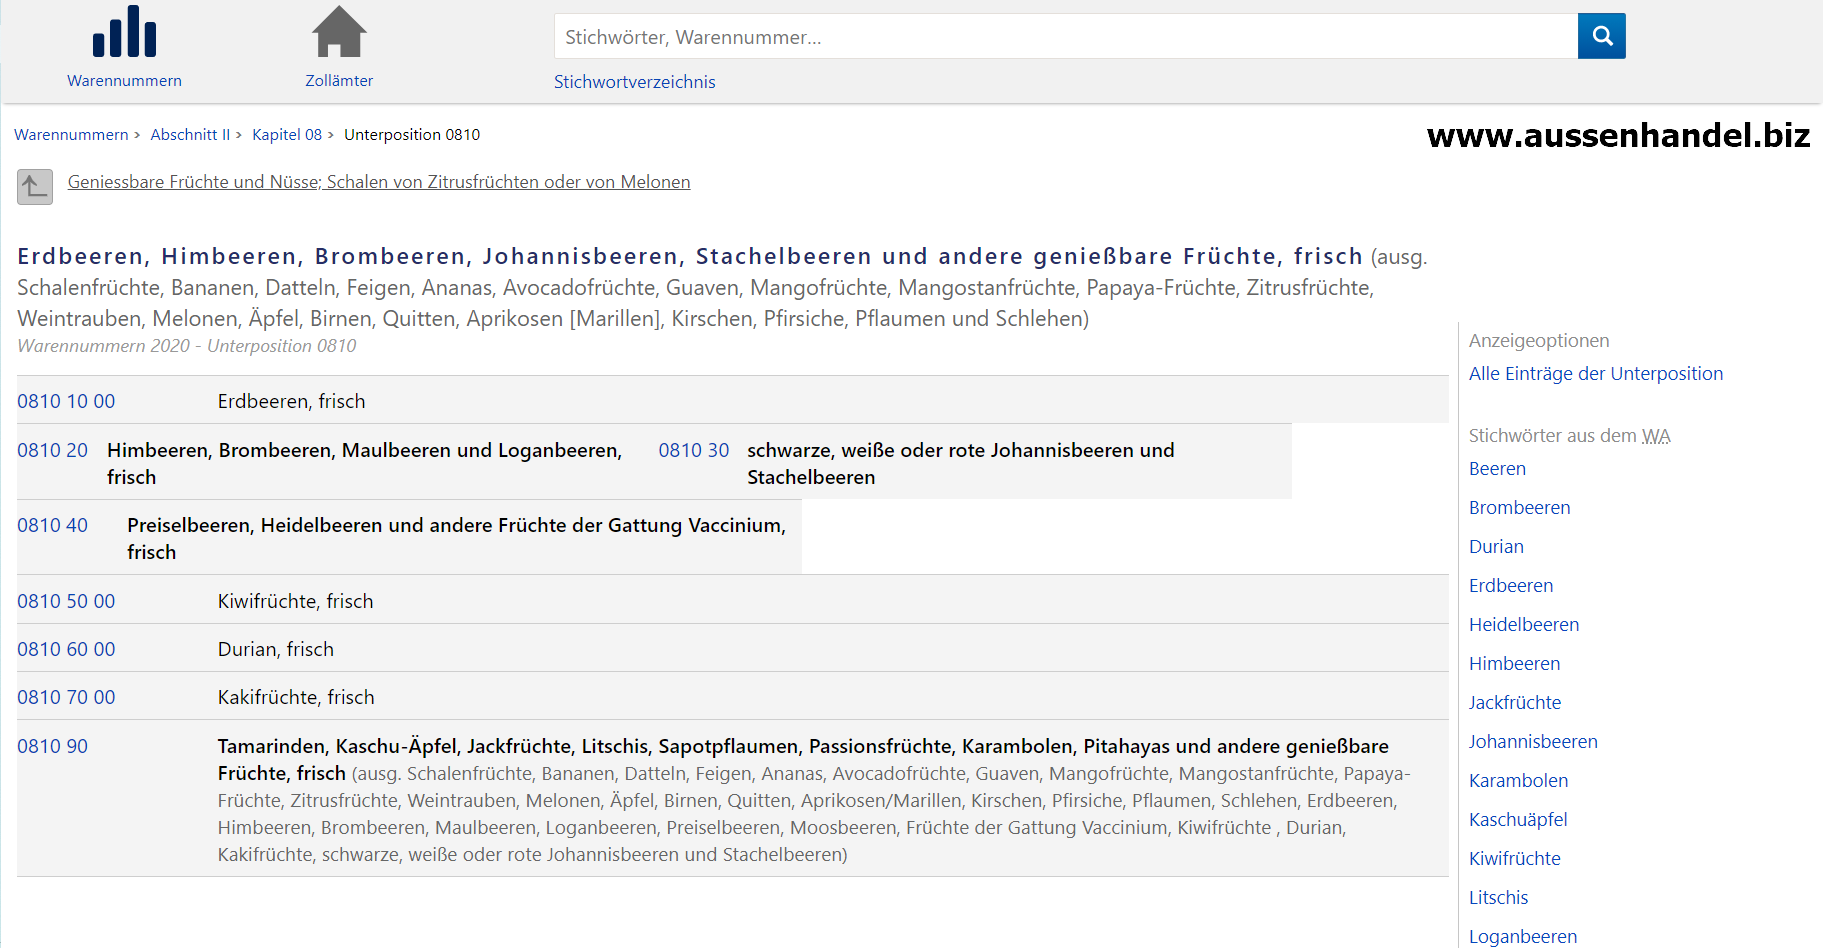
\includegraphics[height=5.5cm]{warennummern}
    \caption{https://aussenhandel.biz}
  \end{figure}
\end{frame}

\begin{frame}
\frametitle{Aufbau WA}
EU-eineitliche Kennzeichnungssystematik
\end{frame}

\begin{frame}
\frametitle{WA: Lebensmittel}
  \begin{figure}[h]
    \centering
    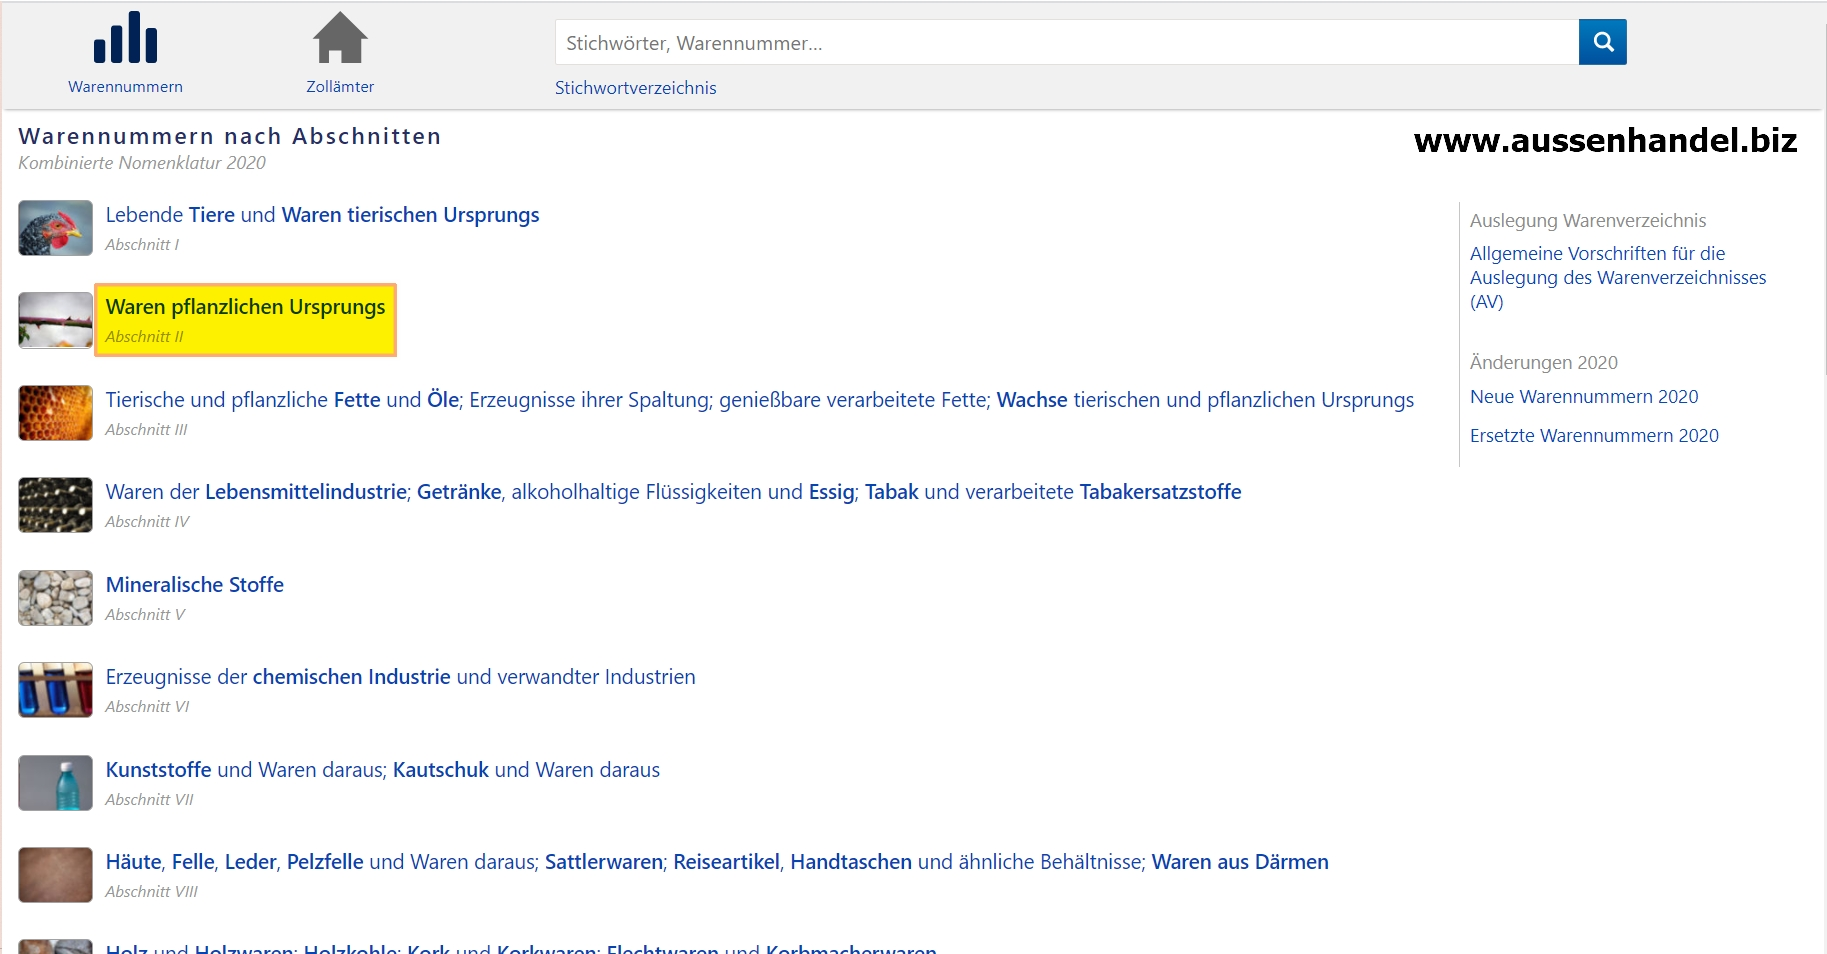
\includegraphics[height=5.5cm]{wa}
    \caption{https://aussenhandel.biz}
  \end{figure}
\end{frame}

\begin{frame}
\frametitle{Beispiel: Spargel}
  \begin{figure}[h]
    \centering
    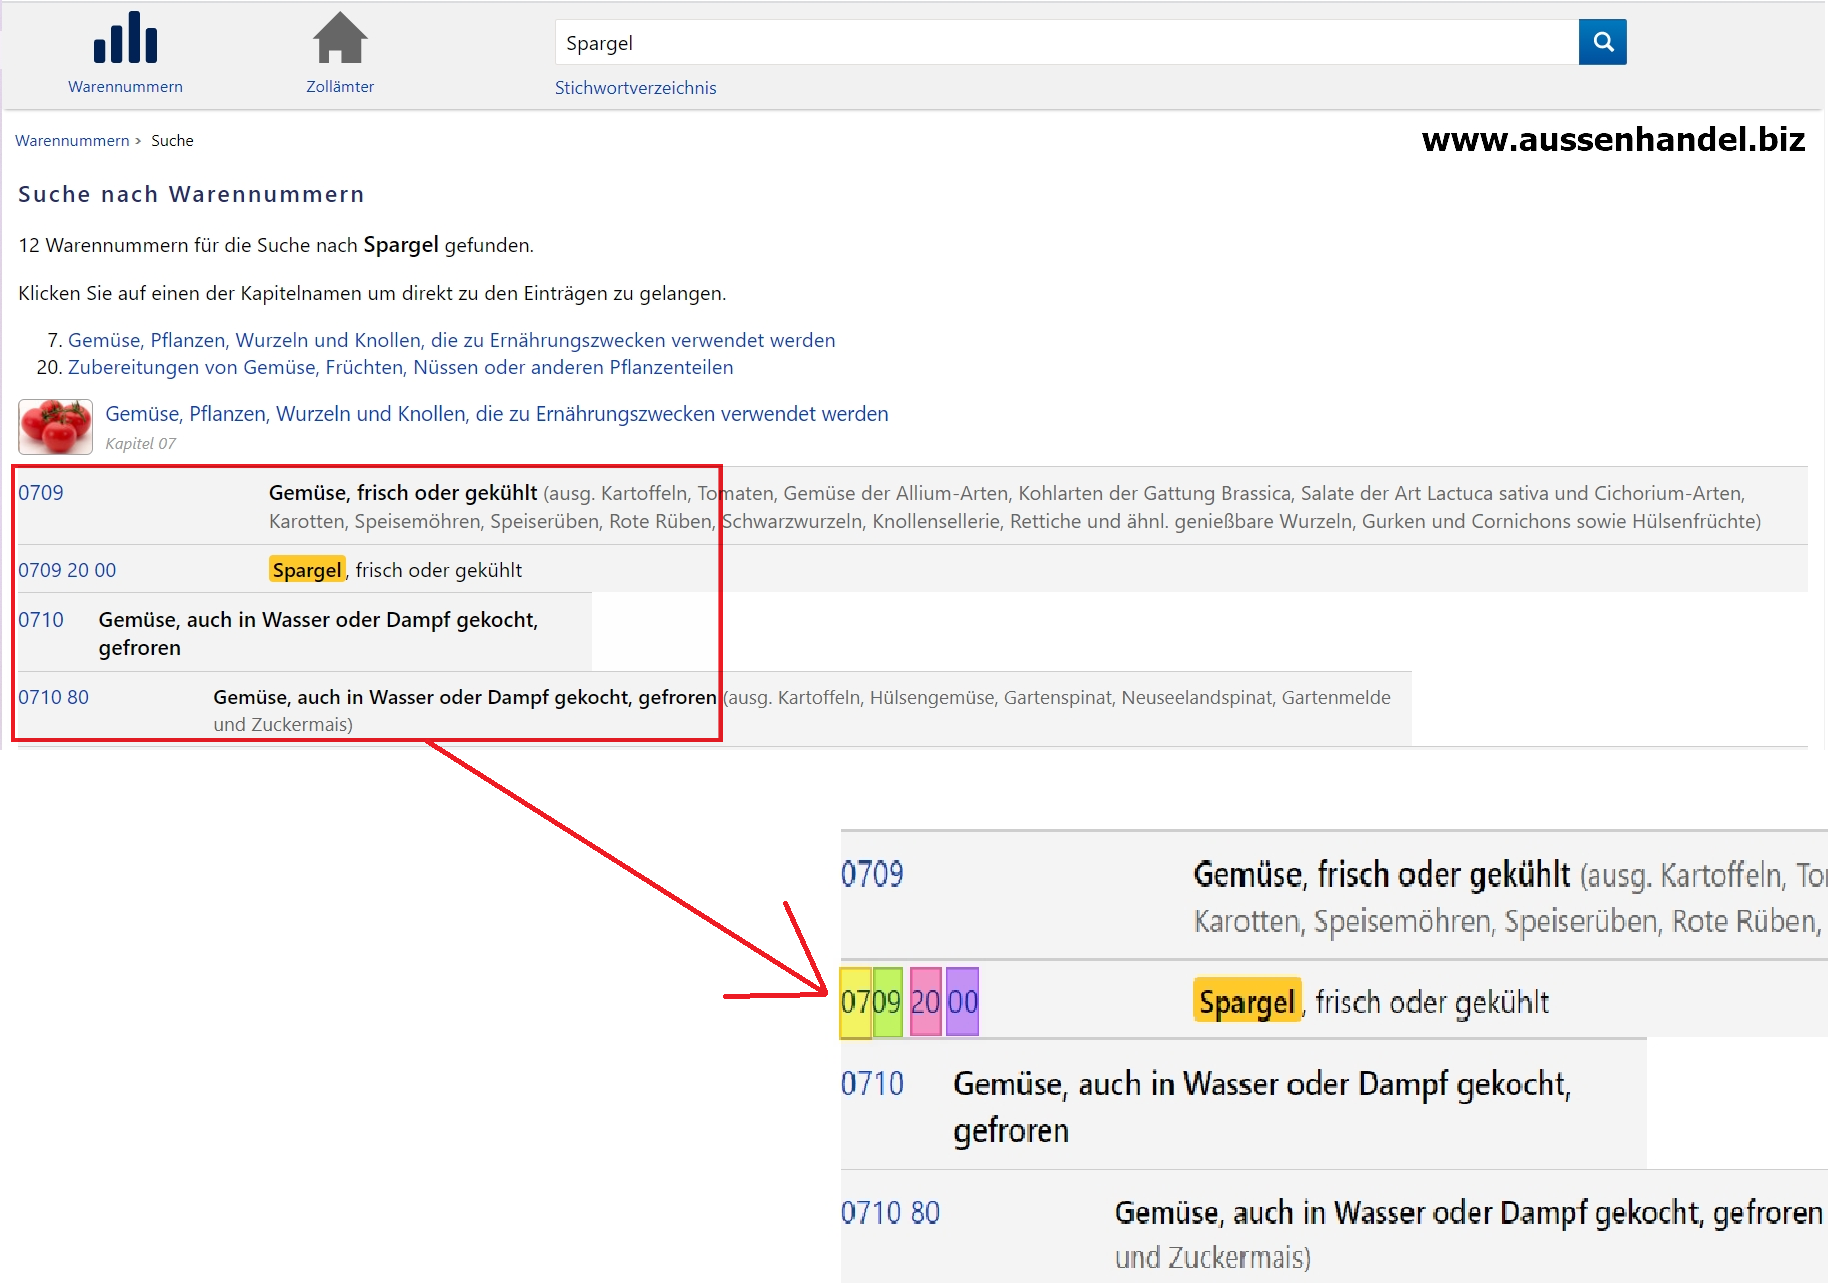
\includegraphics[height=6cm]{wa-spargel}
    \caption{https://aussenhandel.biz}
  \end{figure}
\end{frame}

\begin{frame}
\frametitle{Beispiel: Spargel}
  \begin{figure}[h]
    \centering
    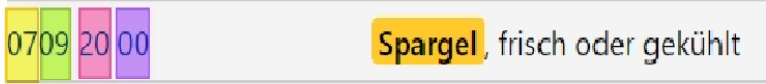
\includegraphics[width=6cm]{wa_spargel}
  \end{figure}

      \begin{itemize}
        \item
07: Gemüse, Pflanzen, Wurzeln und Knollen
        \item
09: Nummer von Gemüse, frisch oder gekühlt
        \item
20: Nummer von Ware Spargel
        \item
00: Keine Unterkategorien
      \end{itemize}
\end{frame}

\section{Wirtschaftliche Theorie} % jörg
\begin{frame}
	\begin{center}
		{\Huge Wirtschaftliche Theorie}
	\end{center}
\end{frame}

\begin{frame}
\frametitle{Knappheit}
  \begin{itemize}
    \item
  Knappheit liegt vor, wenn die Nachfrage größer ist als
  das Angebot.
    \item
      \textbf{Zufällige Knappheit}: Unvorhersehbare Schwankungen
  im Angebot von Obst oder Gemüse.
      \begin{itemize}
        \item
  Hervorgerufen durch schlechte Ernten wegen Dürre oder
  Unwetter.
\item
Knappe Güter können zu erheblichen Preissteigerungen führen.
  \end{itemize}
      \end{itemize}
\end{frame}

\begin{frame}
\frametitle{Angebot}
  \begin{itemize}
    \item
Angebot bezeichnet die Menge eines Gutes, die die
Hersteller zu einem bestimmten Preis produzieren
können.
      \begin{itemize}
        \item
  Das Angebot abhängig von (Produktionsfaktoren, dem Stand
  der Produktionstechnik und den Erwartungen an den Markt).
      \end{itemize}
  \end{itemize}
\end{frame}

\begin{frame}
\frametitle{Nachfrage}
  \begin{itemize}
    \item
Nachfrage ist die Menge an Gütern, die die
Konsumenten zu einem bestimmten Preis kaufen wollen.

      \begin{itemize}
        \item
Hauptkriterien für den Kauf: Menge des Gutes, die Höhe des
eigenen Einkommens, persönlicher Geschmack und der Preis ähnlicher Produkte.
      \end{itemize}
  \end{itemize}
\end{frame}

\begin{frame}
\frametitle{steigendes Angebot}
  \begin{figure}[h]
    \centering
    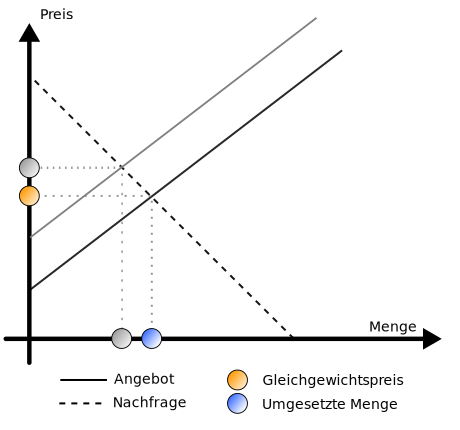
\includegraphics[height=6cm]{steigendes_angebot}
    \caption{https://de.wikipedia.org/wiki/Marktgleichgewicht}
  \end{figure}
\end{frame}
\begin{frame}
\frametitle{Economies of scale}

\begin{columns}
    \begin{column}{0.5\textwidth}
  \begin{figure}[h]
    \centering
      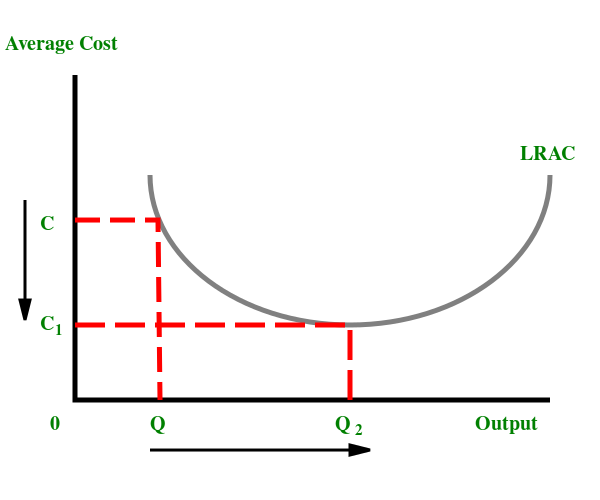
\includegraphics[width=0.9\textwidth]{economies_of_scale}
      \caption{https://napkinfinance.com/wp-content/uploads/2016/11/Economies-of-Scale-final.jpg}
  \end{figure}
    \end{column}
    \begin{column}{0.5\textwidth}
    \begin{itemize}
    \item
  Mit Ausweitung der zu
  erwirtschaftenden Gütern,
  wird eine größere Menge
  dieser, auf die
  gleichbleibenden Fixkosten
  aufgeteilt.
\item
  Somit sind die Fixkosten pro
  Stück geringer.

    \end{itemize}
    \end{column}
\end{columns}
\end{frame}


\section{Datenbeschaffung}
\begin{frame}
	\begin{center}
		{\Huge Datenbeschaffung und -bereinigung}
	\end{center}
\end{frame}

\section{Datenbeschaffung}
\begin{frame}
	\begin{center}
		{\Huge Datenbeschaffung}
	\end{center}
\end{frame}

\begin{frame}
	\frametitle{Beginn der Datensuche}
		\begin{itemize}
			\item statistische Jahrbuch des Bundesministeriums für Ernährung und Landwirtschaft (BMEL)
		\end{itemize}

		\begin{figure}[!tbp]
  			\centering
			\begin{minipage}[b]{0.3\textwidth}
			\caption{https://www.bmel-statistik.de/archiv/statistisches-jahrbuch/}
			
\includegraphics[scale=0.15, width=\textwidth]{1_BMEL-Statistisches_Jahrbuch}
  			\end{minipage}
  		\hfill
			\begin{minipage}[b]{0.4\textwidth}
    				\caption{https://www.bmel-statistik.de/archiv/statistischer-monatsbericht/}
				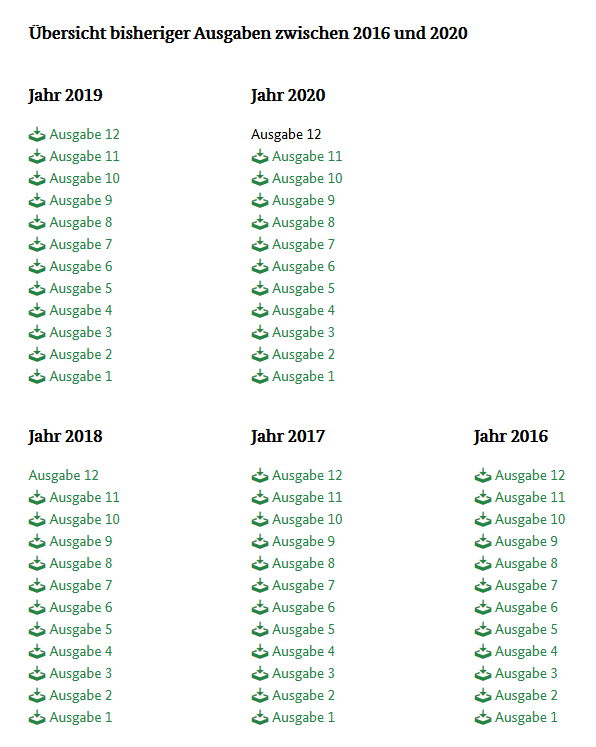
\includegraphics[scale=0.4,width=\textwidth]{2_Monatsberichte}
  			\end{minipage}
		\end{figure}
\end{frame}

\begin{frame}
	\frametitle{Beginn der Datensuche}
	\begin{figure}[h]
	\caption{Statistischer Monatsbericht von Juni 2020 (Seite 489)}
	\centering
	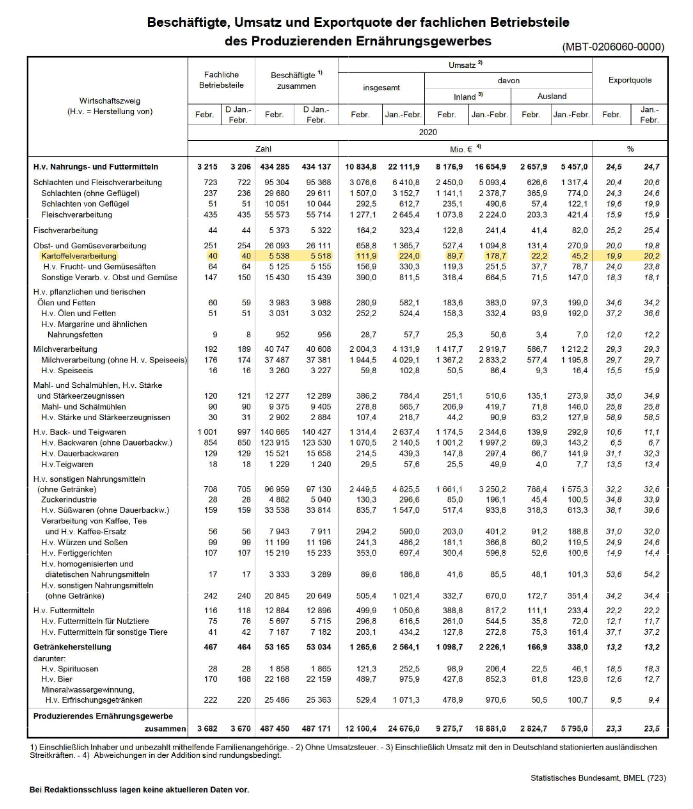
\includegraphics[scale=0.5]{3_Beispieltabelle}
	\end{figure}
\end{frame}

\begin{frame}
	\frametitle{Probleme}
	\begin{figure}[h]
		\caption{unvollständige Auflistung}
		\centering
		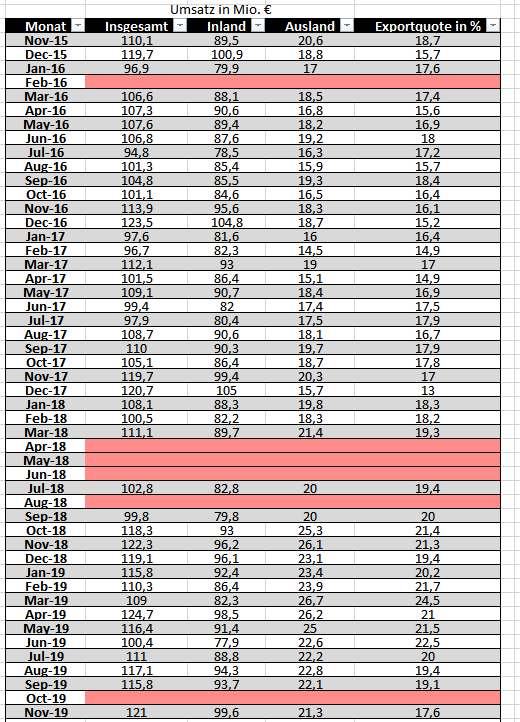
\includegraphics[scale=0.3]{4_Monatsberichte_unvoll}
	\end{figure}
\end{frame}

\begin{frame}
	\frametitle{statista.com}
	\begin{figure}[h]
		\caption{https://de.statista.com/statistik/daten/studie/206617/umfrage/importmenge-von-obst-und-gemuese-nach-deutschland/}
		\centering
		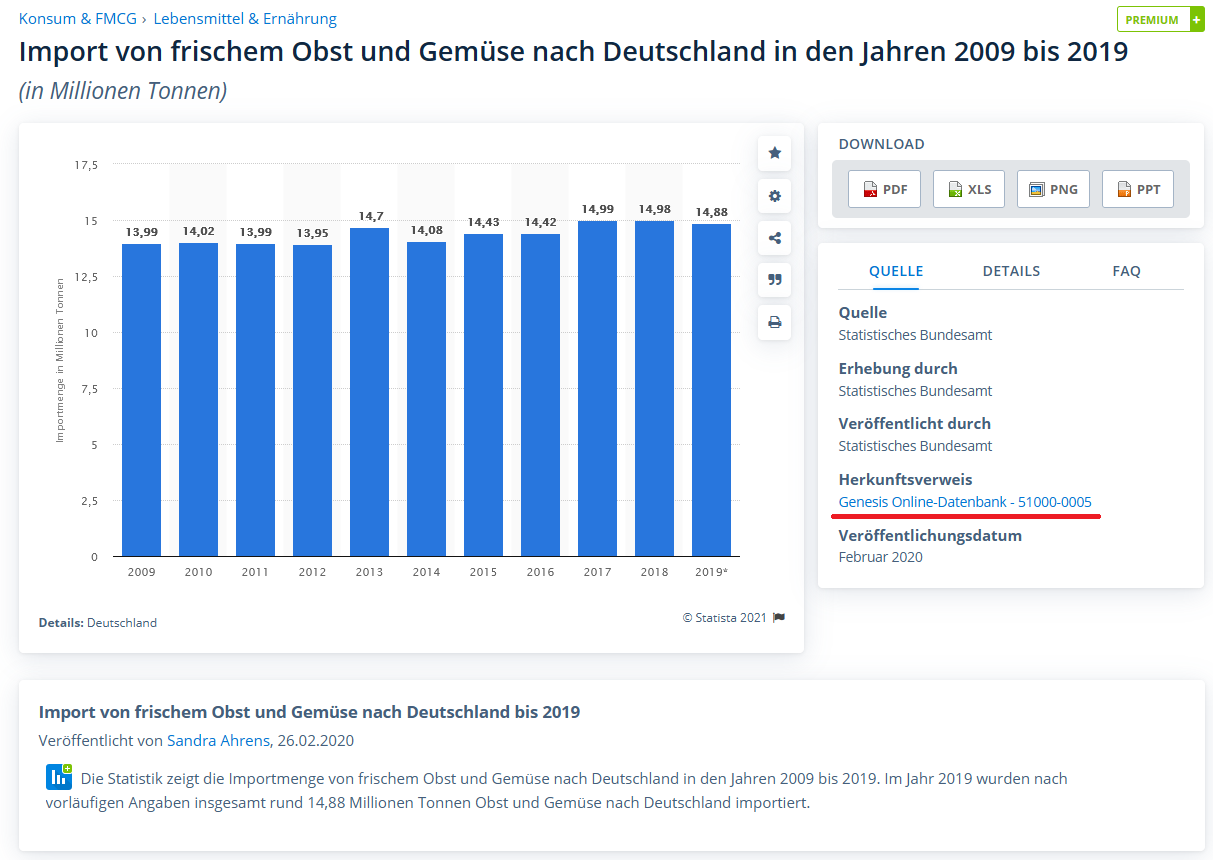
\includegraphics[scale=0.3]{5_Destatis_Report_highlightet}
	\end{figure}
\end{frame}

\begin{frame}
	\frametitle{Lösungen}
	\begin{figure}[h]
		\caption{https://www-genesis.destatis.de/genesis/online}
		\centering
		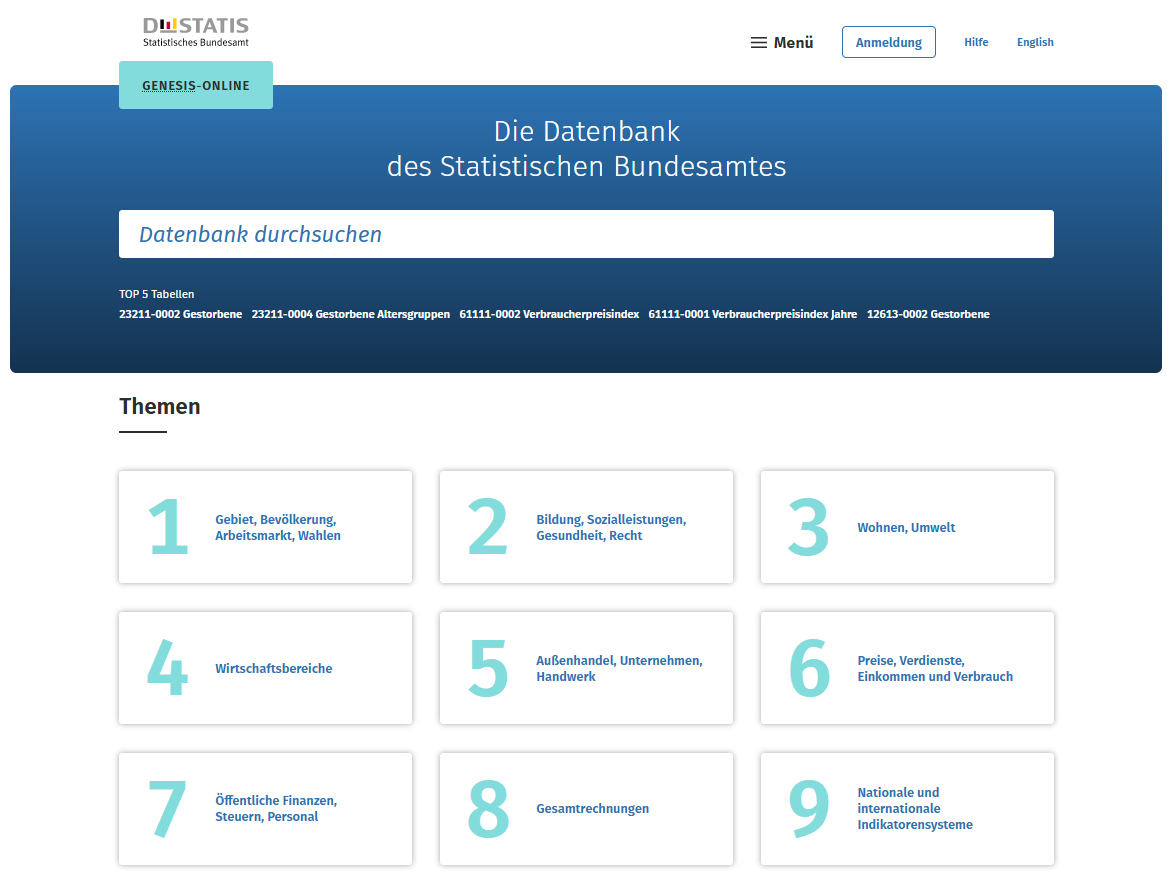
\includegraphics[scale=0.15]{6_Denesis_Destatis}
	\end{figure}
\end{frame}

\begin{frame}
	\frametitle{Lösung}
	\begin{figure}[h]
		\caption{https://www-genesis.destatis.de/genesis/online?operation=find\& suchanweisung\_ language=de\& query=51000\# abreadcrumb}
		\centering
		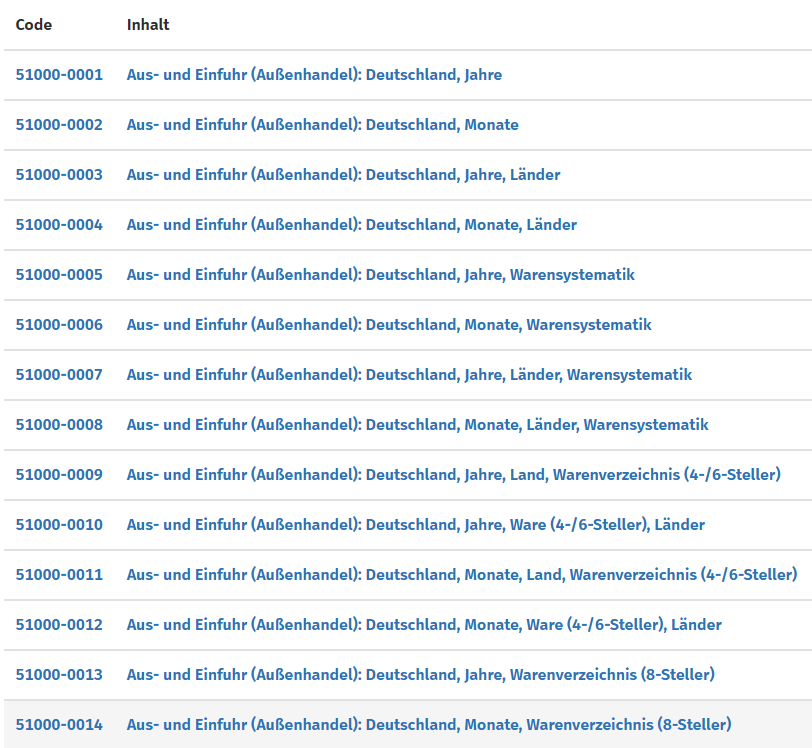
\includegraphics[scale=0.2]{8_Tabellen_codes}
	\end{figure}
\end{frame}

\begin{frame}
	\frametitle{}
	\begin{figure}[h]
		\caption{https://www-genesis.destatis.de/genesis/online?operation=abruftabelleBearbeiten\& levelindex=0\& levelid=1610310696241\& auswahloperation=abruftabelleAuspraegungAuswaehlen\& auswahlverzeichnis=ordnungsstruktur\& auswahlziel=werteabruf\& code=51000-0014\& auswahltext=\& wertauswahl=256\& wertauswahl=253\& wertauswahl=257\& wertauswahl=254\& transponieren=1610310713629\# astructure}
		\centering
		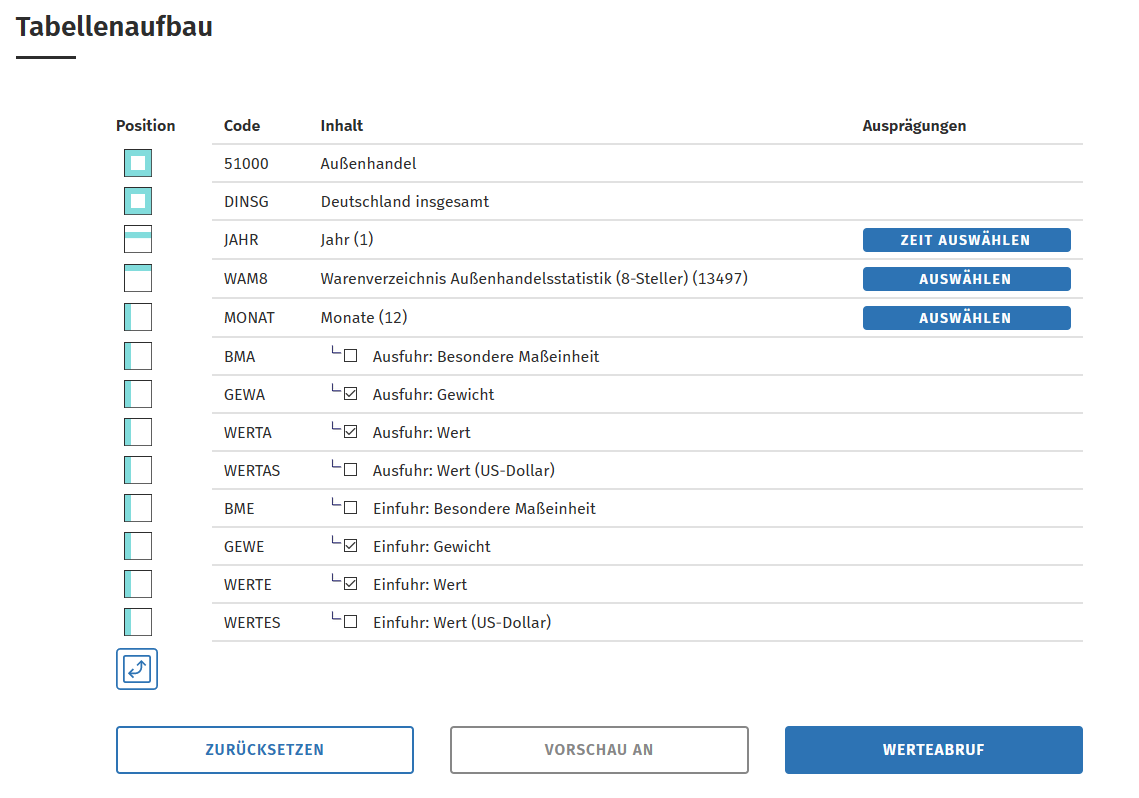
\includegraphics[scale=0.25]{9_Tabellanaufbau}
	\end{figure}
\end{frame}

\begin{frame}
	\frametitle{Lösung}
	\begin{itemize}
		\item Import in Excel
		\item anschließend grobe Aufbereitungsschritte in kleinere CSV-Dateien
	\end{itemize}
\end{frame}

\section{Datenverarbeitung}
\begin{frame}
	\begin{center}
		{\Huge Datenverarbeitung}
	\end{center}
\end{frame}

\begin{frame}
	\frametitle{Standardachsen}
	x-Achse:
	\begin{itemize}
		\item kombiniert
		\item jährlich (Durchschnitt)
		\item monatlich (Durchschnitt)
	\end{itemize}
	y-Achse:
	\begin{itemize}
		\item Gewicht in Tonnen
		\item Volumen in Euro
		\item Volumen pro Gewicht (Euro/Tonne)
	\end{itemize}
\end{frame}

\begin{frame}
	\frametitle{Datenstruktur}
	\begin{figure}[b]
		\centering
		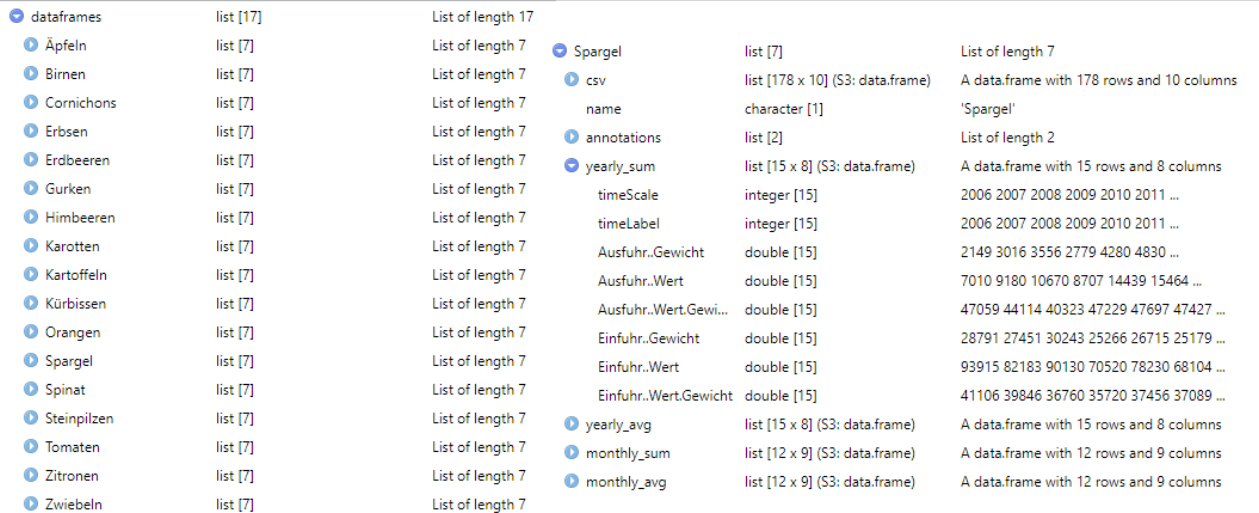
\includegraphics[scale=0.4]{Folie2}
	\end{figure}
\end{frame}

\begin{frame}
	\frametitle{Probleme der Darstellung}
	\begin{itemize}
		\item diskrete Daten an der Abszisse
		\begin{itemize}
			\item falsche Aussagen aus Liniendigramm 
		\end{itemize}
		\item optische Abgrenzung schwierig
		\item Saisons nicht erkennbar
	\end{itemize}

	\begin{figure}[b]
		\centering
		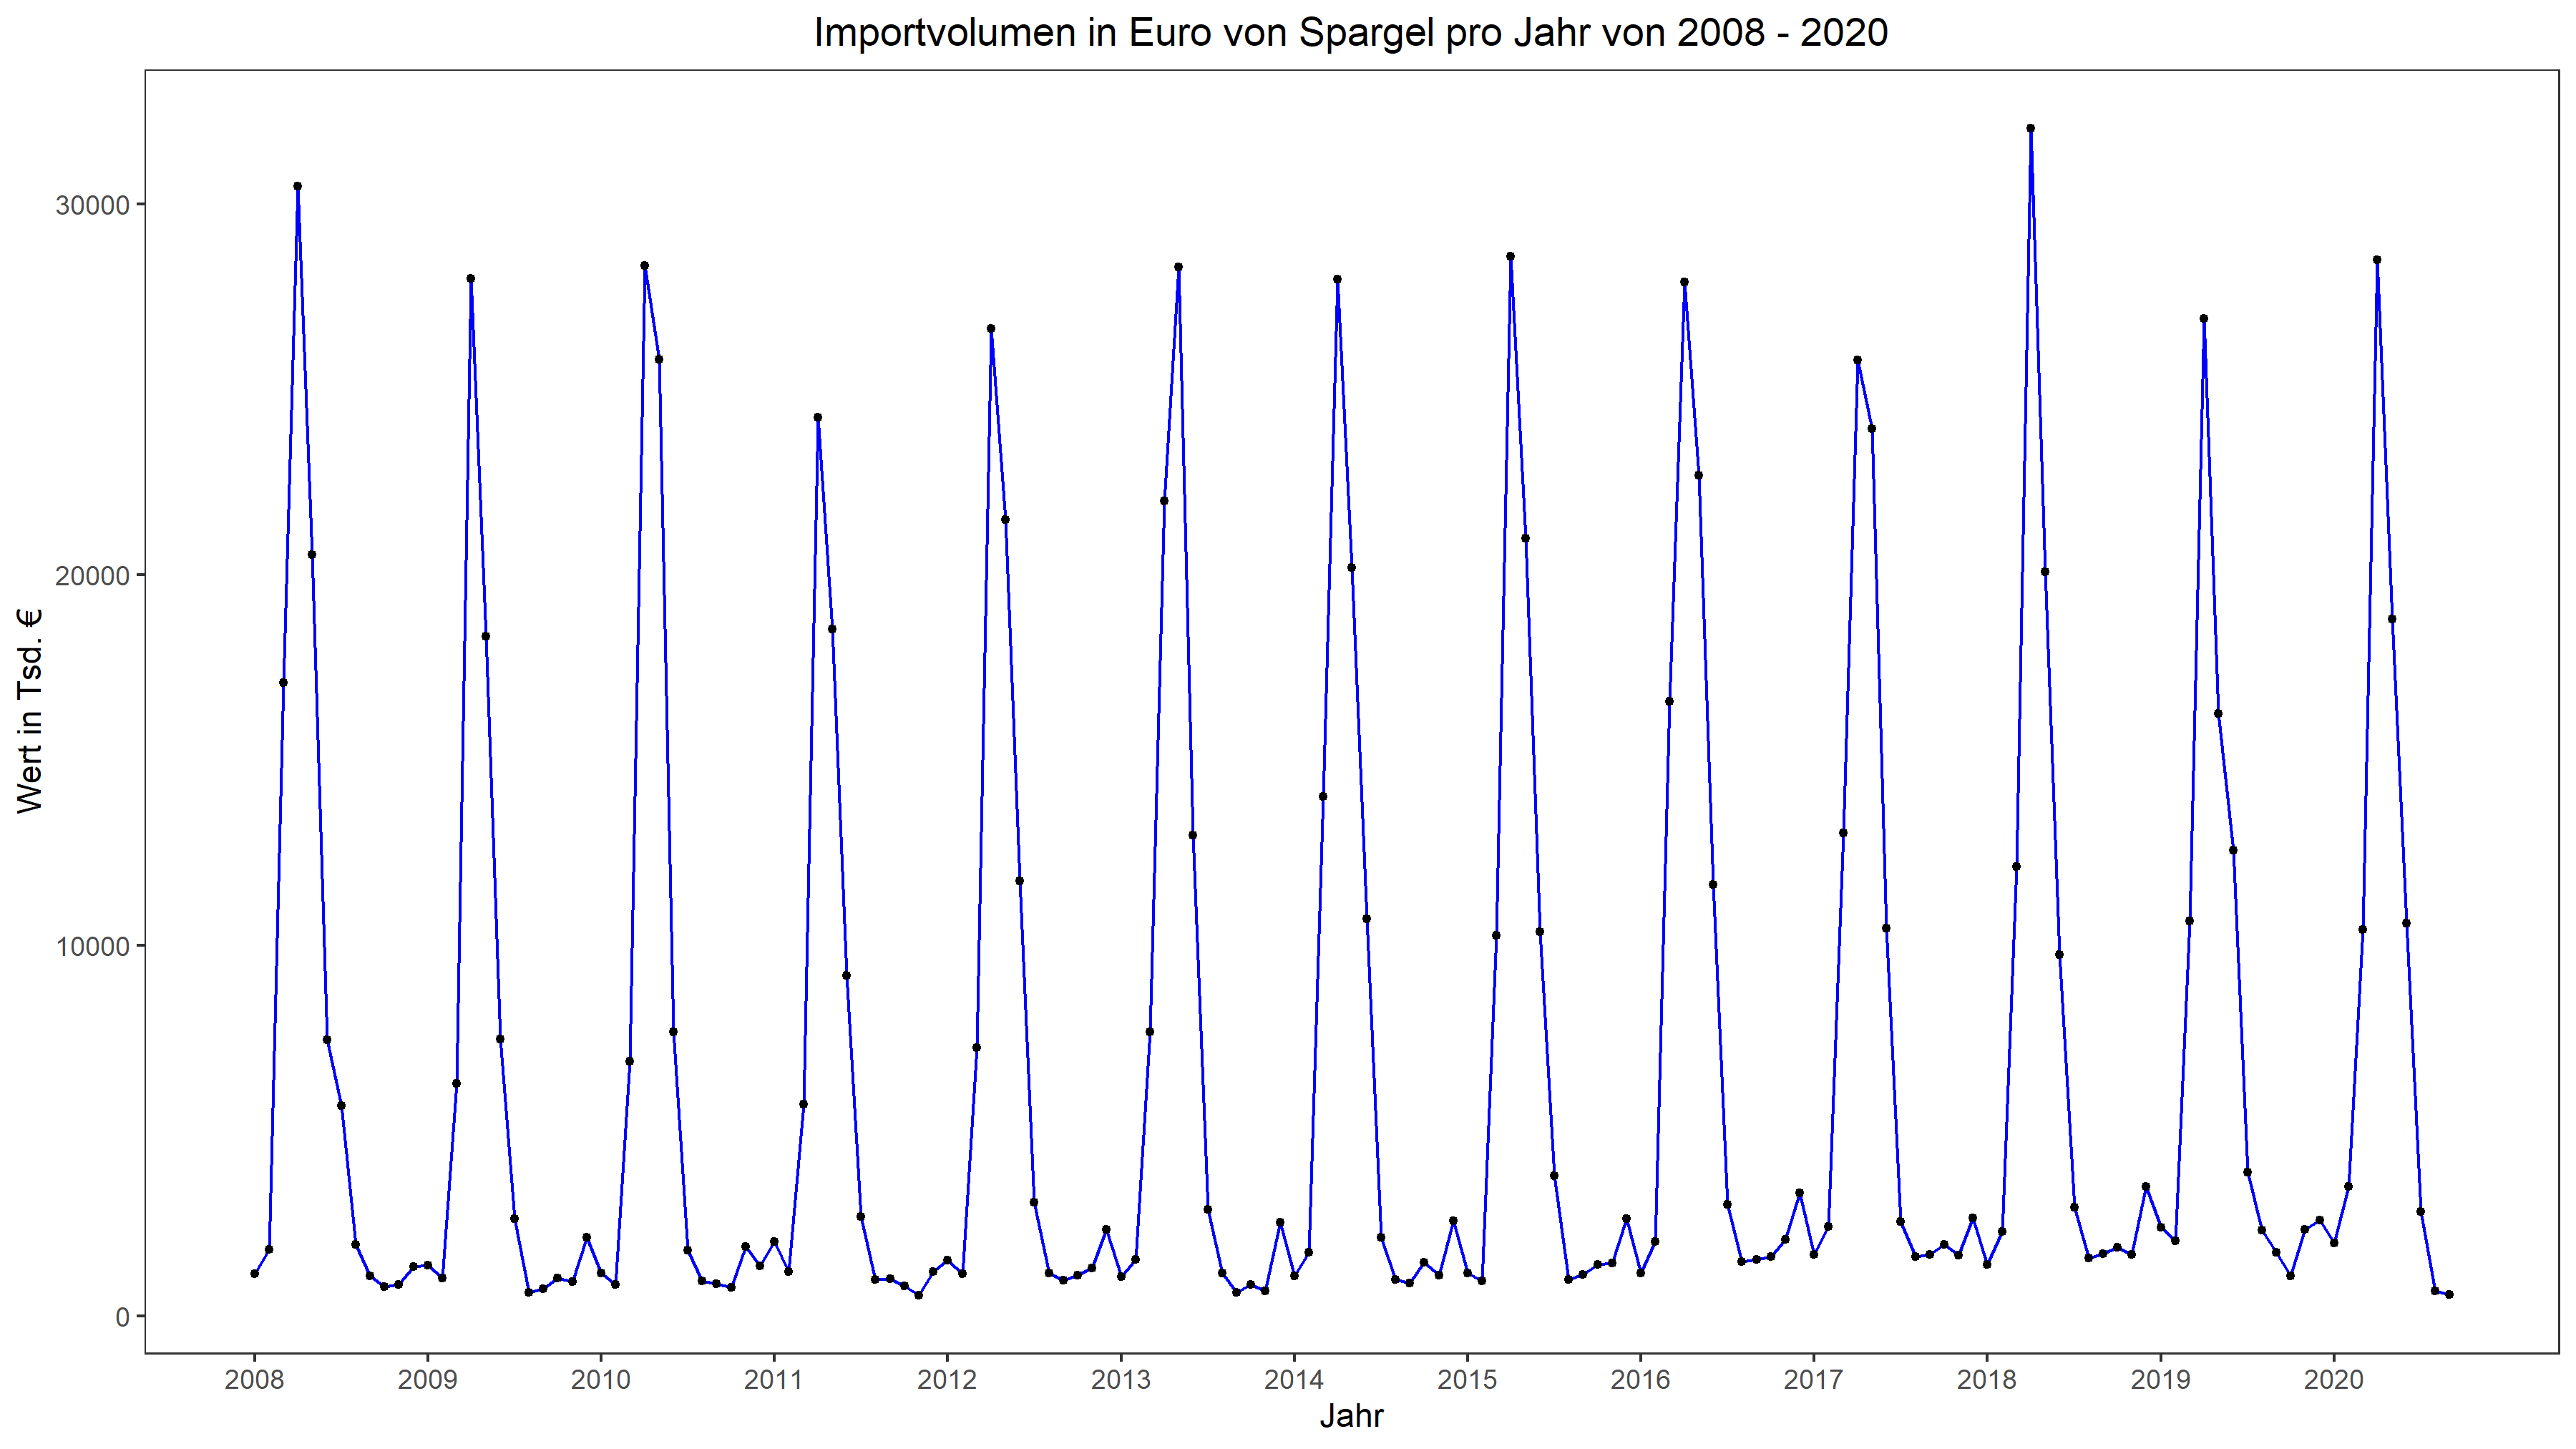
\includegraphics[scale=0.3]{Marco_2_Folie}
	\end{figure}
\end{frame}

\begin{frame}
	\frametitle{Darstellung der Saison}
	\begin{figure}
		\centering
		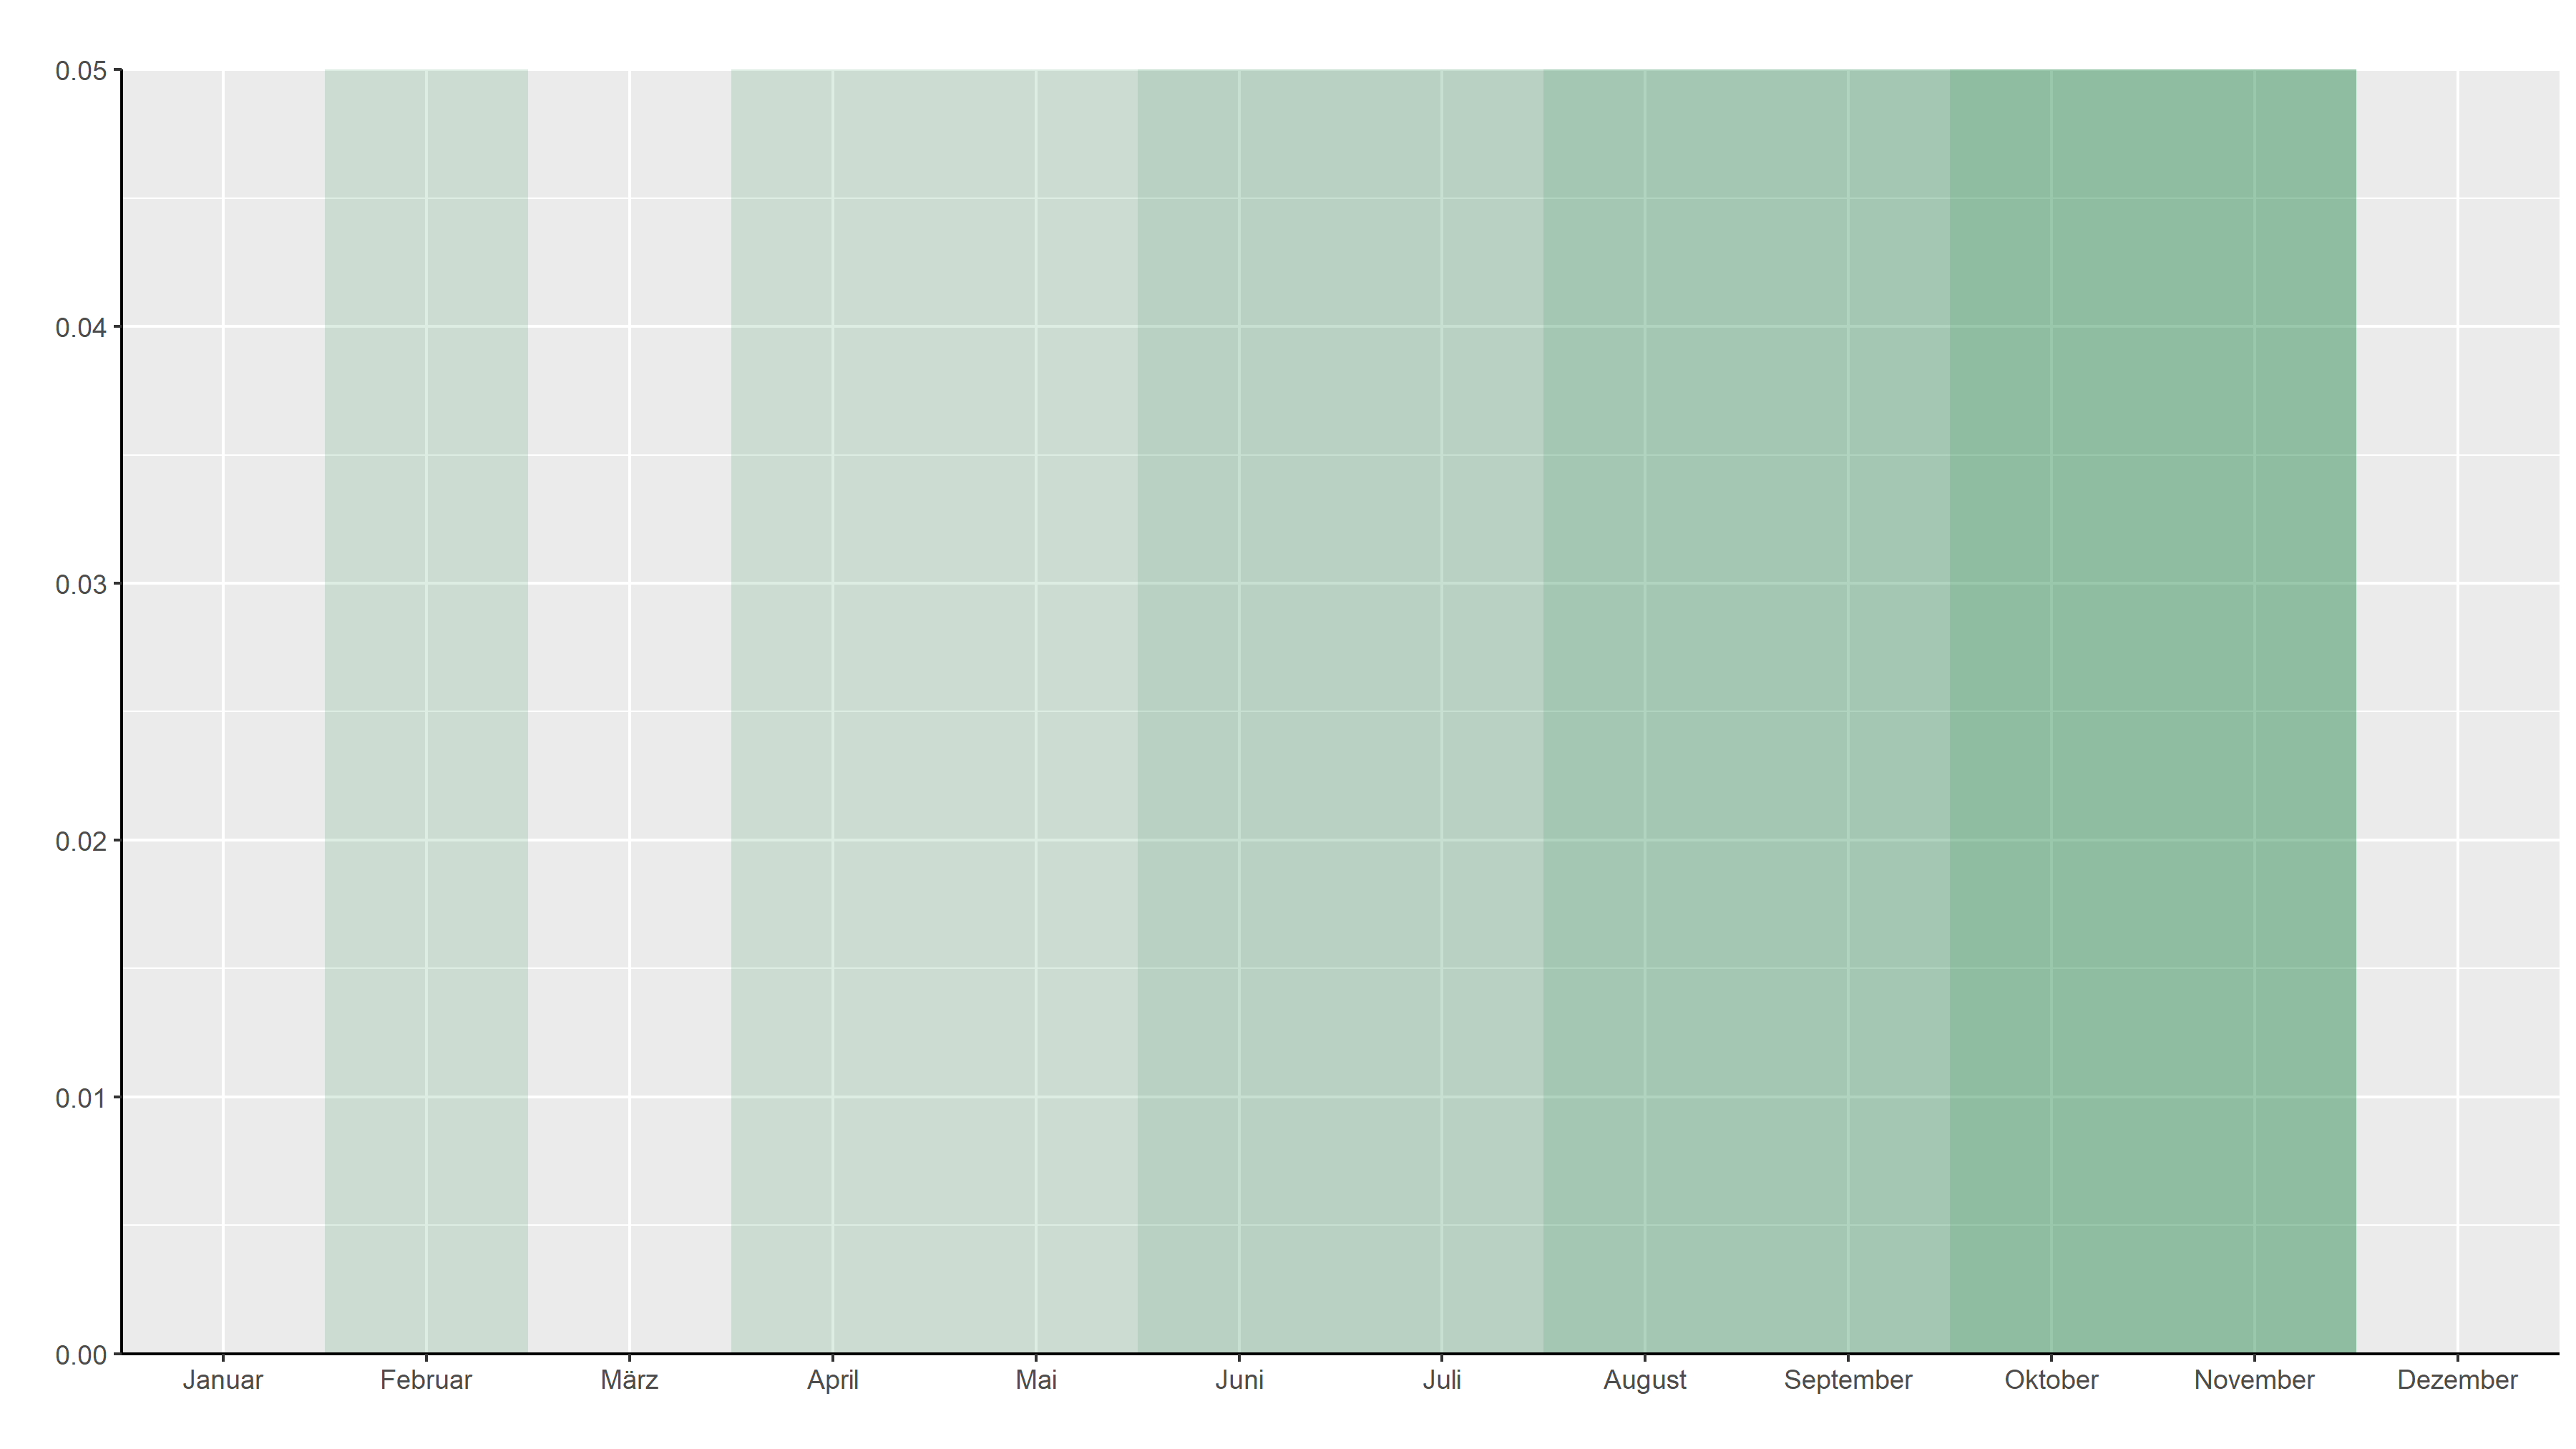
\includegraphics[scale=0.35]{Marco_3_Folie}
	\end{figure}
\end{frame}

\begin{frame}
	\frametitle{optimierte Darstellung}
	\begin{figure}[b]
		\centering
		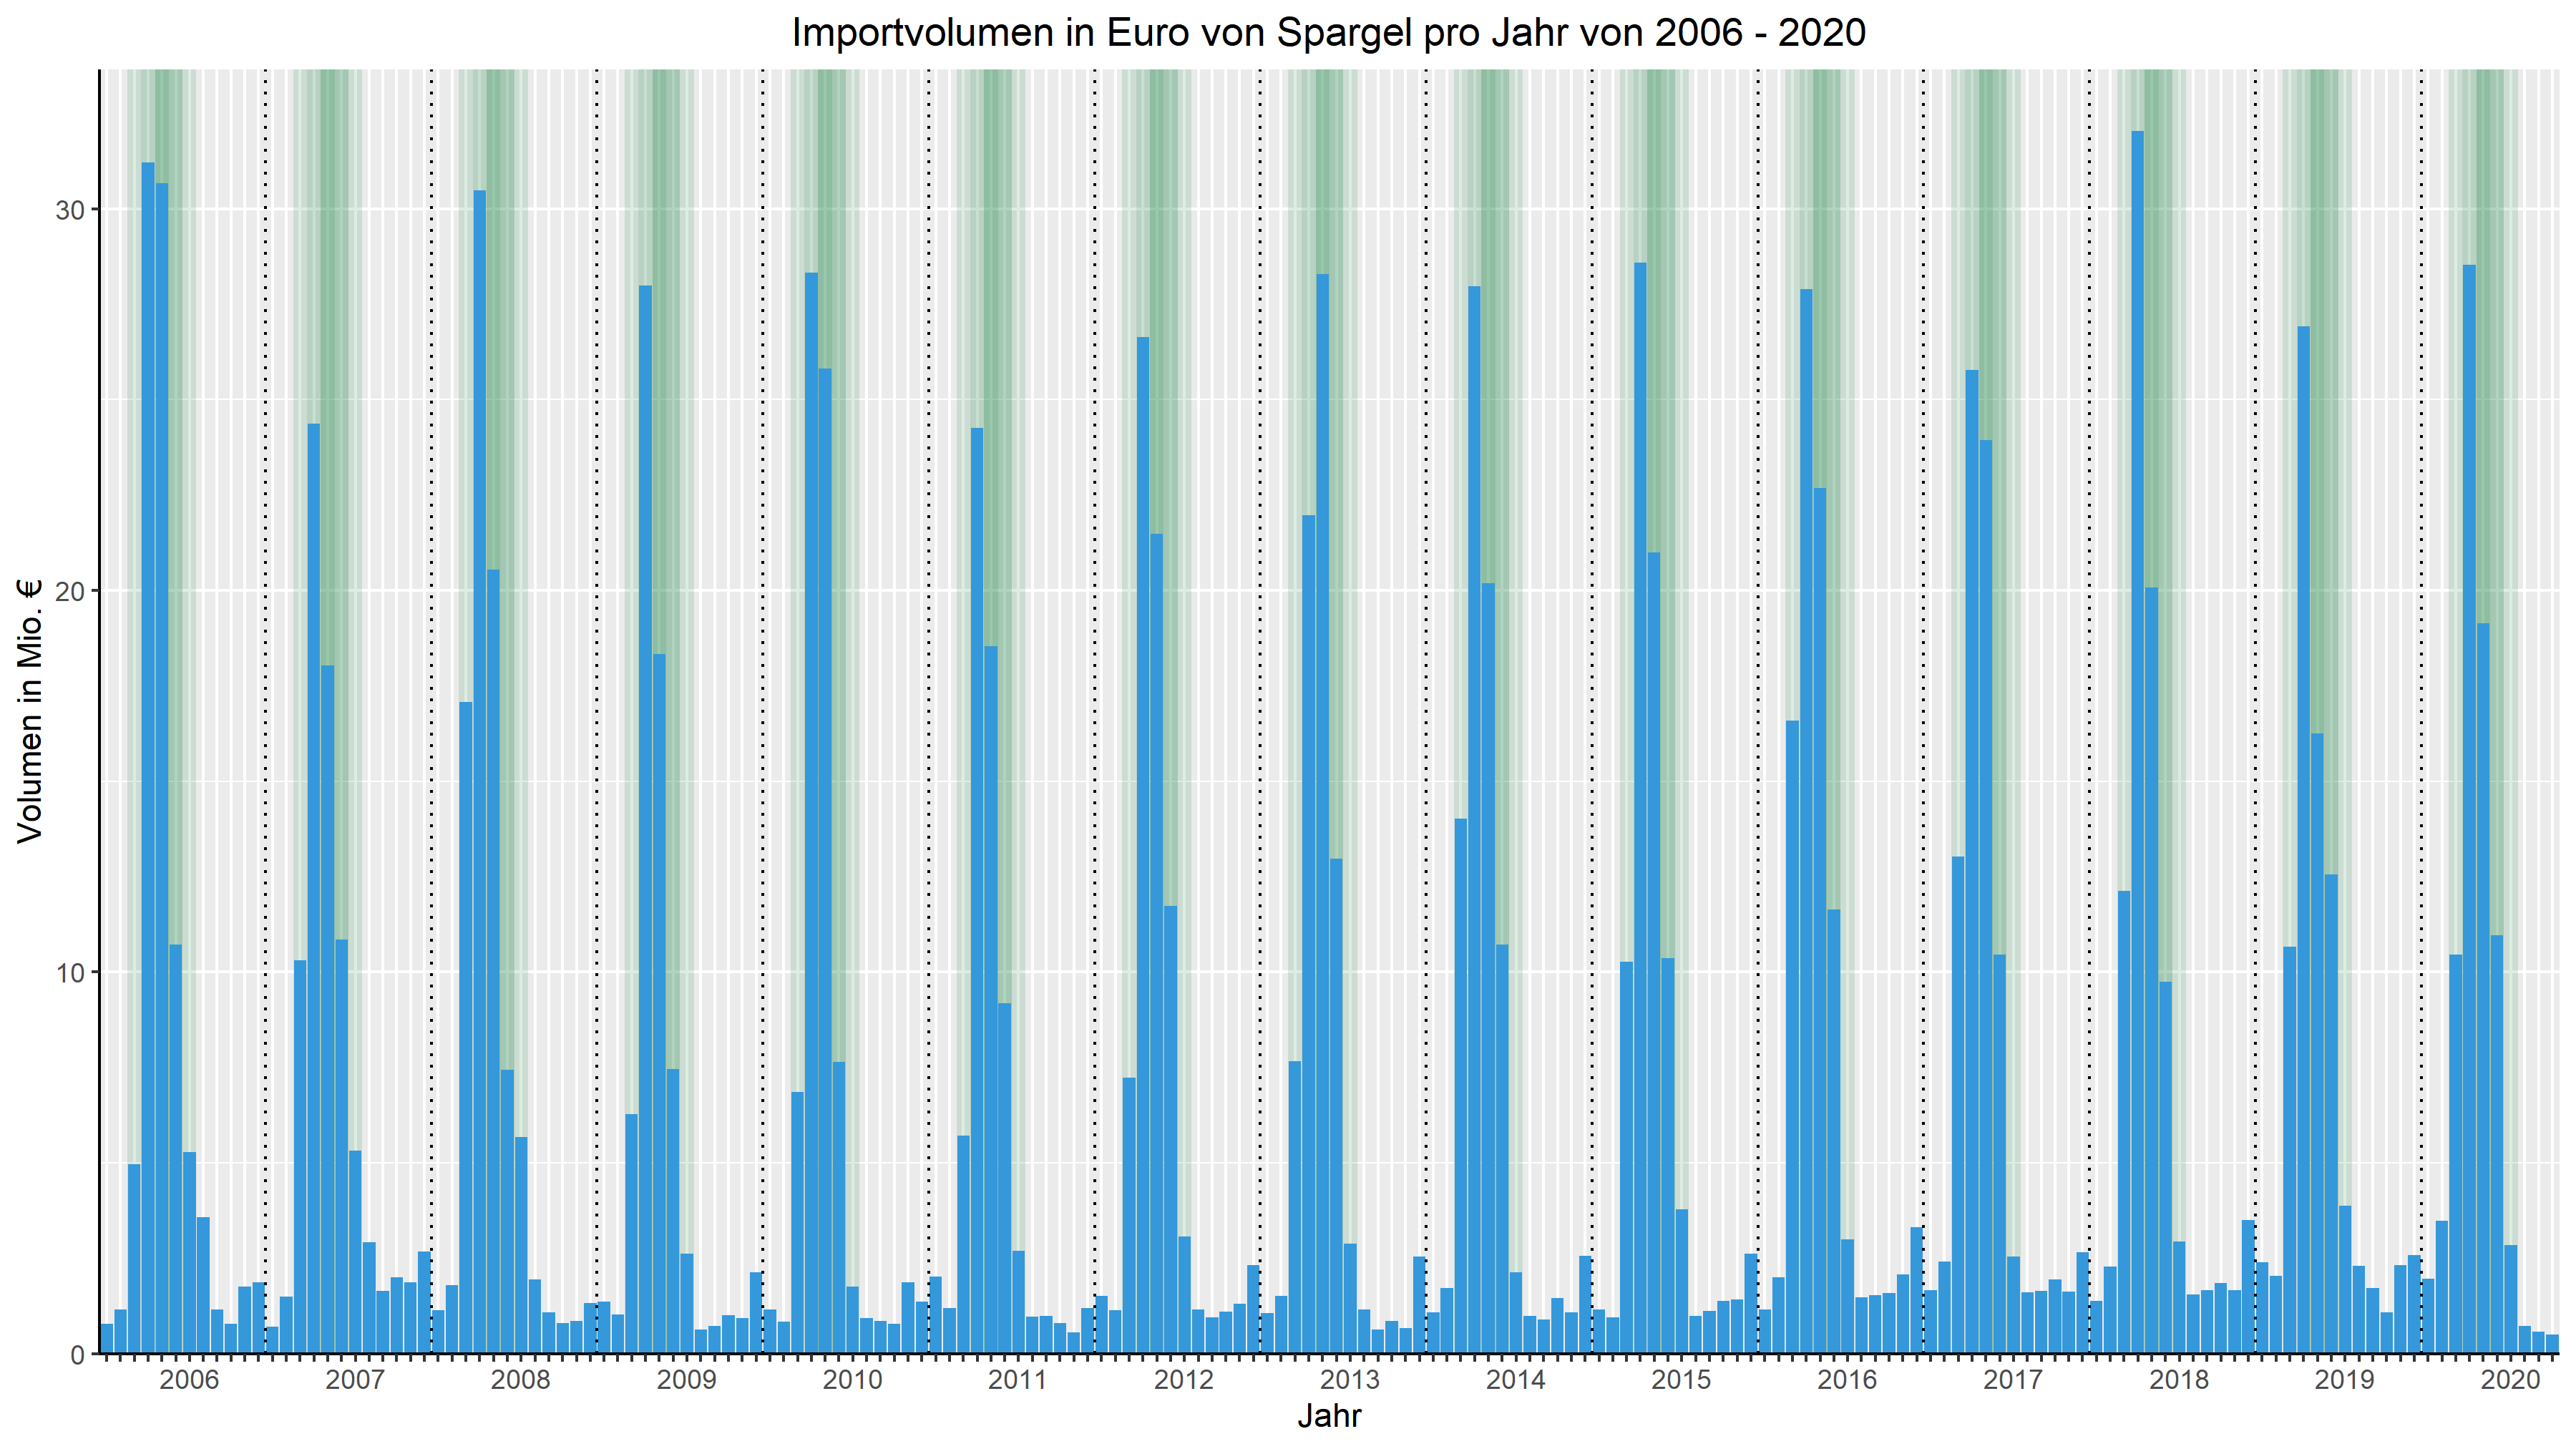
\includegraphics[scale=0.35]{Marco_4_Folie}
	\end{figure}
\end{frame}

\begin{frame}
	\frametitle{Probleme Boxplot}
	\begin{figure}[b]
		\centering
		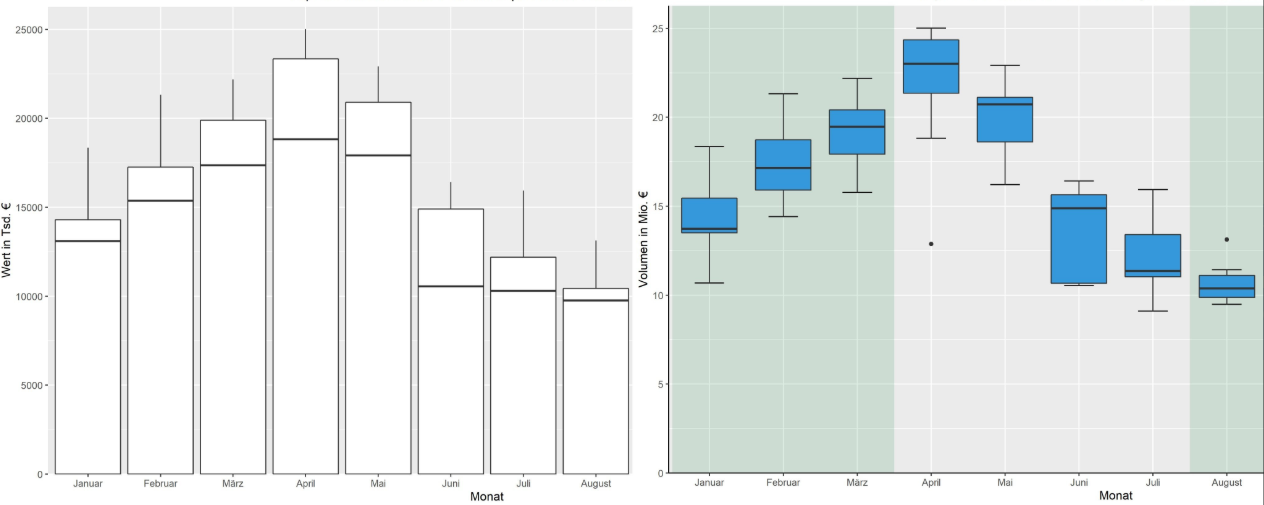
\includegraphics[scale=0.4]{boxplots-folie-5}
	\end{figure}
\end{frame}

\begin{frame}
	\frametitle{Boxplot - Ausreißer}
	\begin{figure}[b]
		\centering
		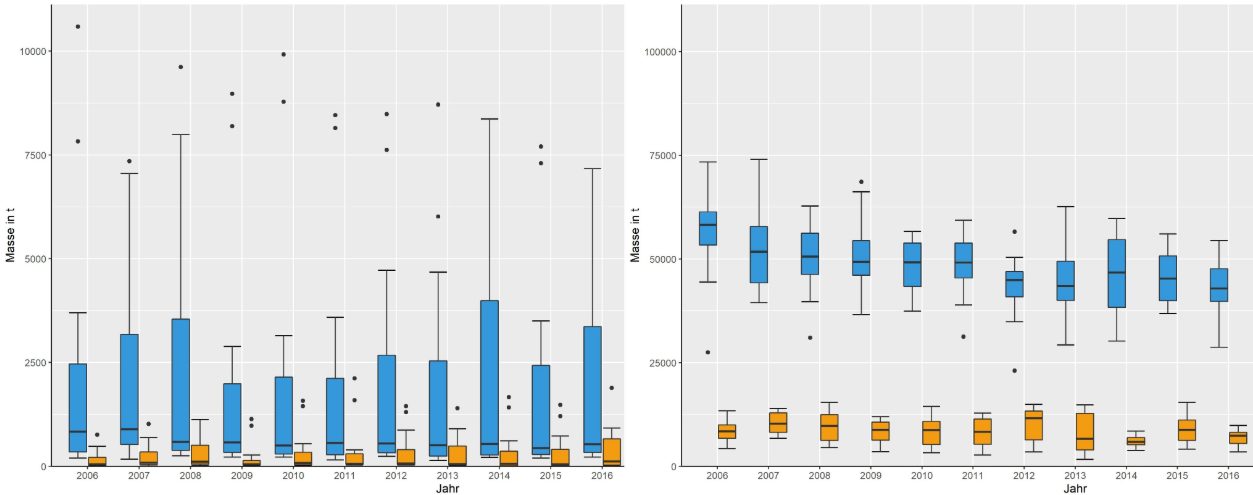
\includegraphics[scale=0.4]{boxplot-prob-gesamt}
	\end{figure}
\end{frame}

\section{Sichtung}
\begin{frame}
	\begin{center}
		{\Huge explorative Datensichtung}
	\end{center}
\end{frame}

% jonathan
\begin{frame}
\frametitle{Äpfel}
  \begin{figure}[h]
    \centering
    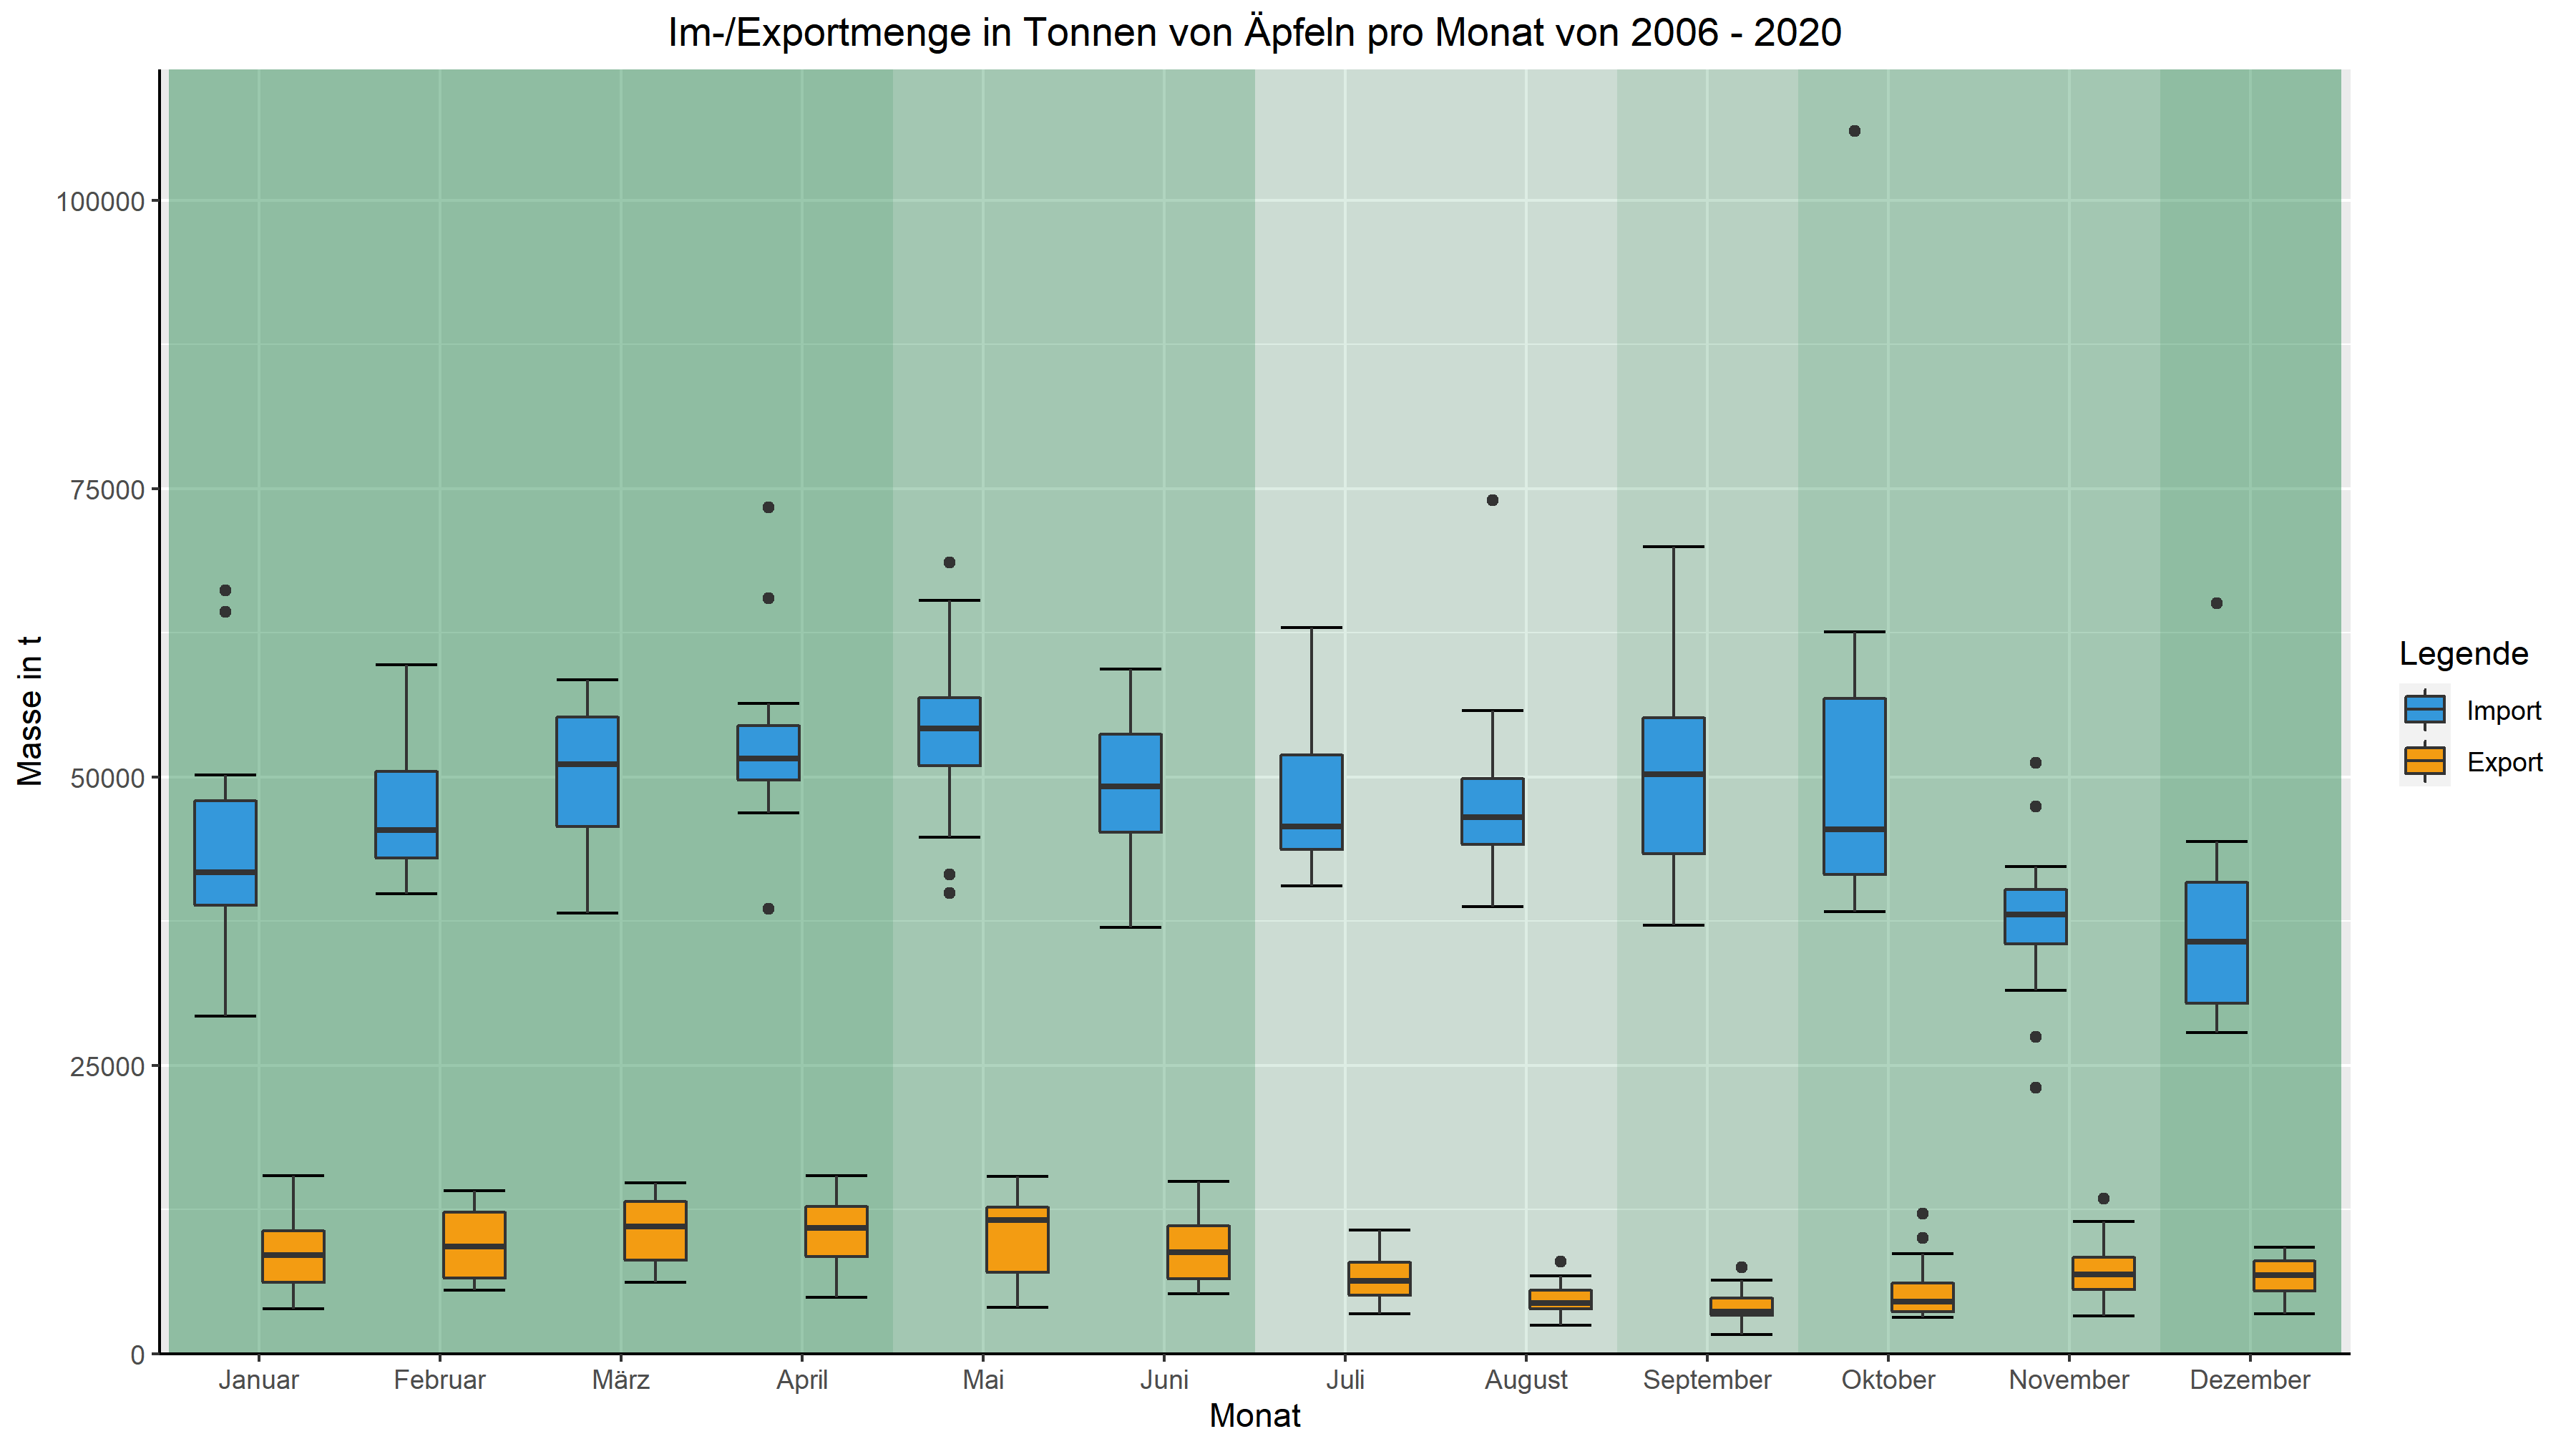
\includegraphics[height=6cm]{0_apfel_markt}
  \end{figure}
\end{frame}

\begin{frame}
\frametitle{Äpfel}
  \begin{figure}[h]
    \centering
    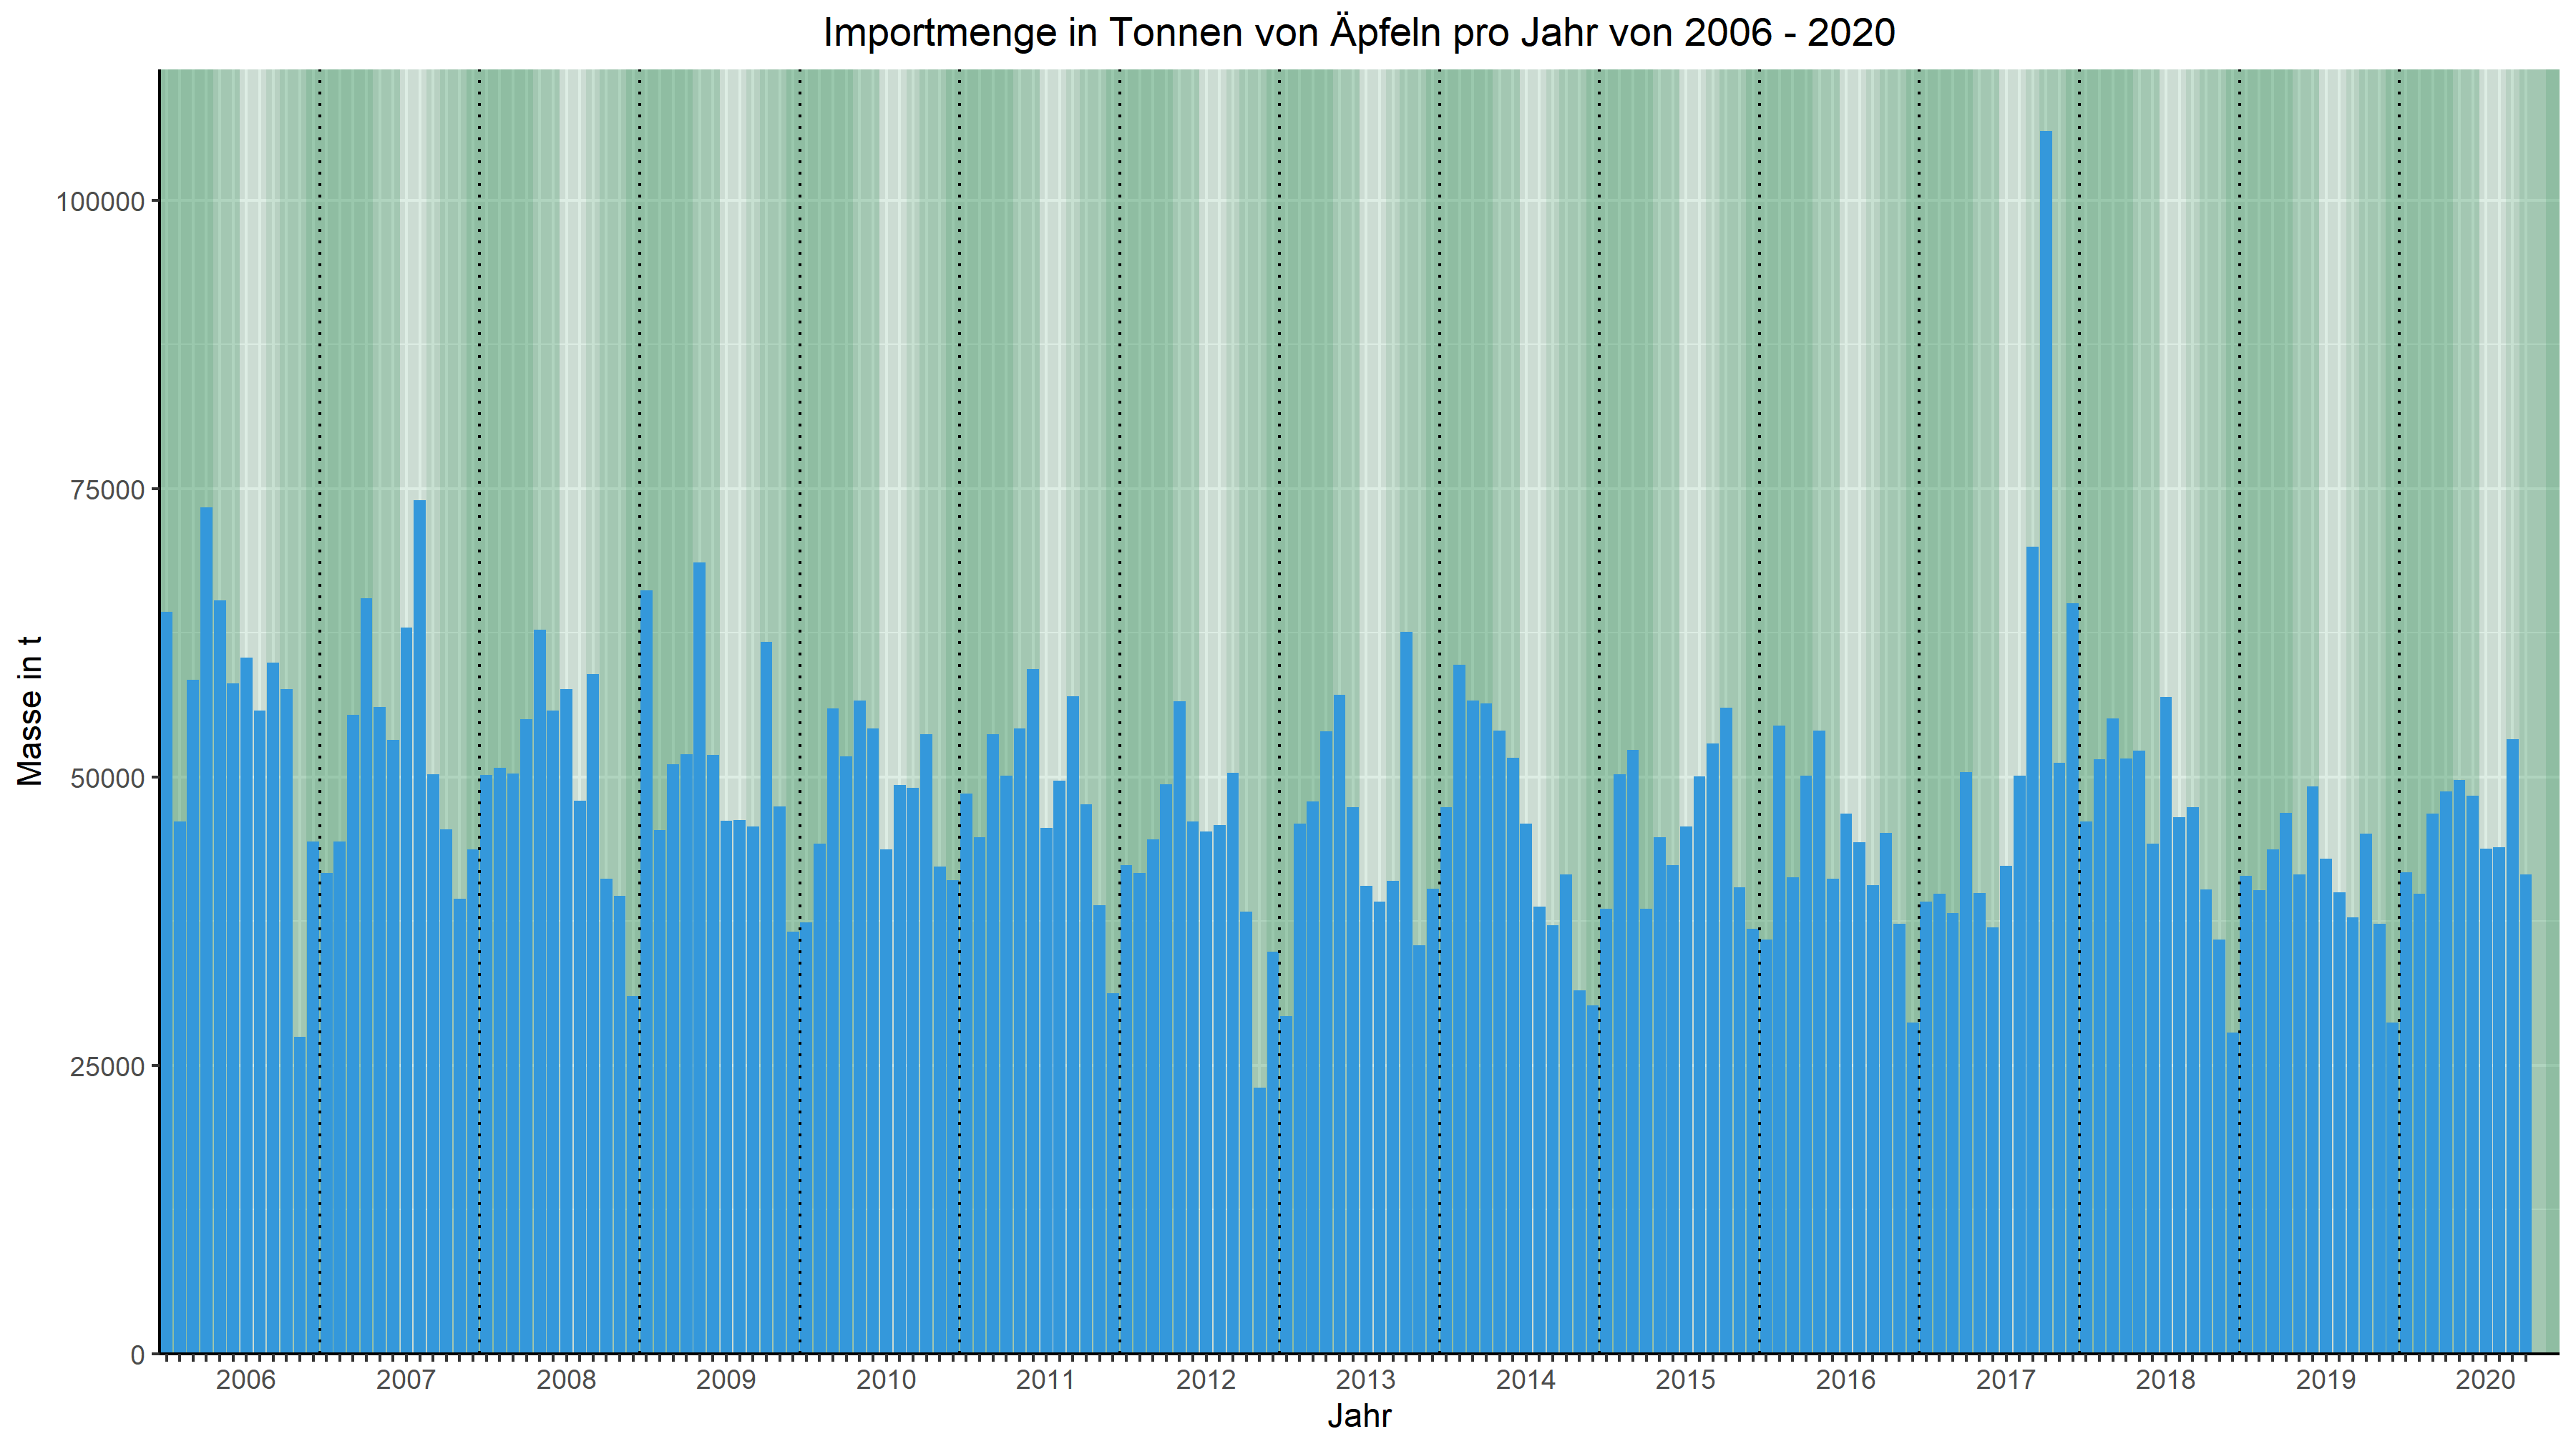
\includegraphics[height=6cm]{0_apfel_import}
  \end{figure}
\end{frame}

\begin{frame}
\frametitle{Äpfel}
  \begin{figure}[h]
    \hbox{\hspace{-1cm}
    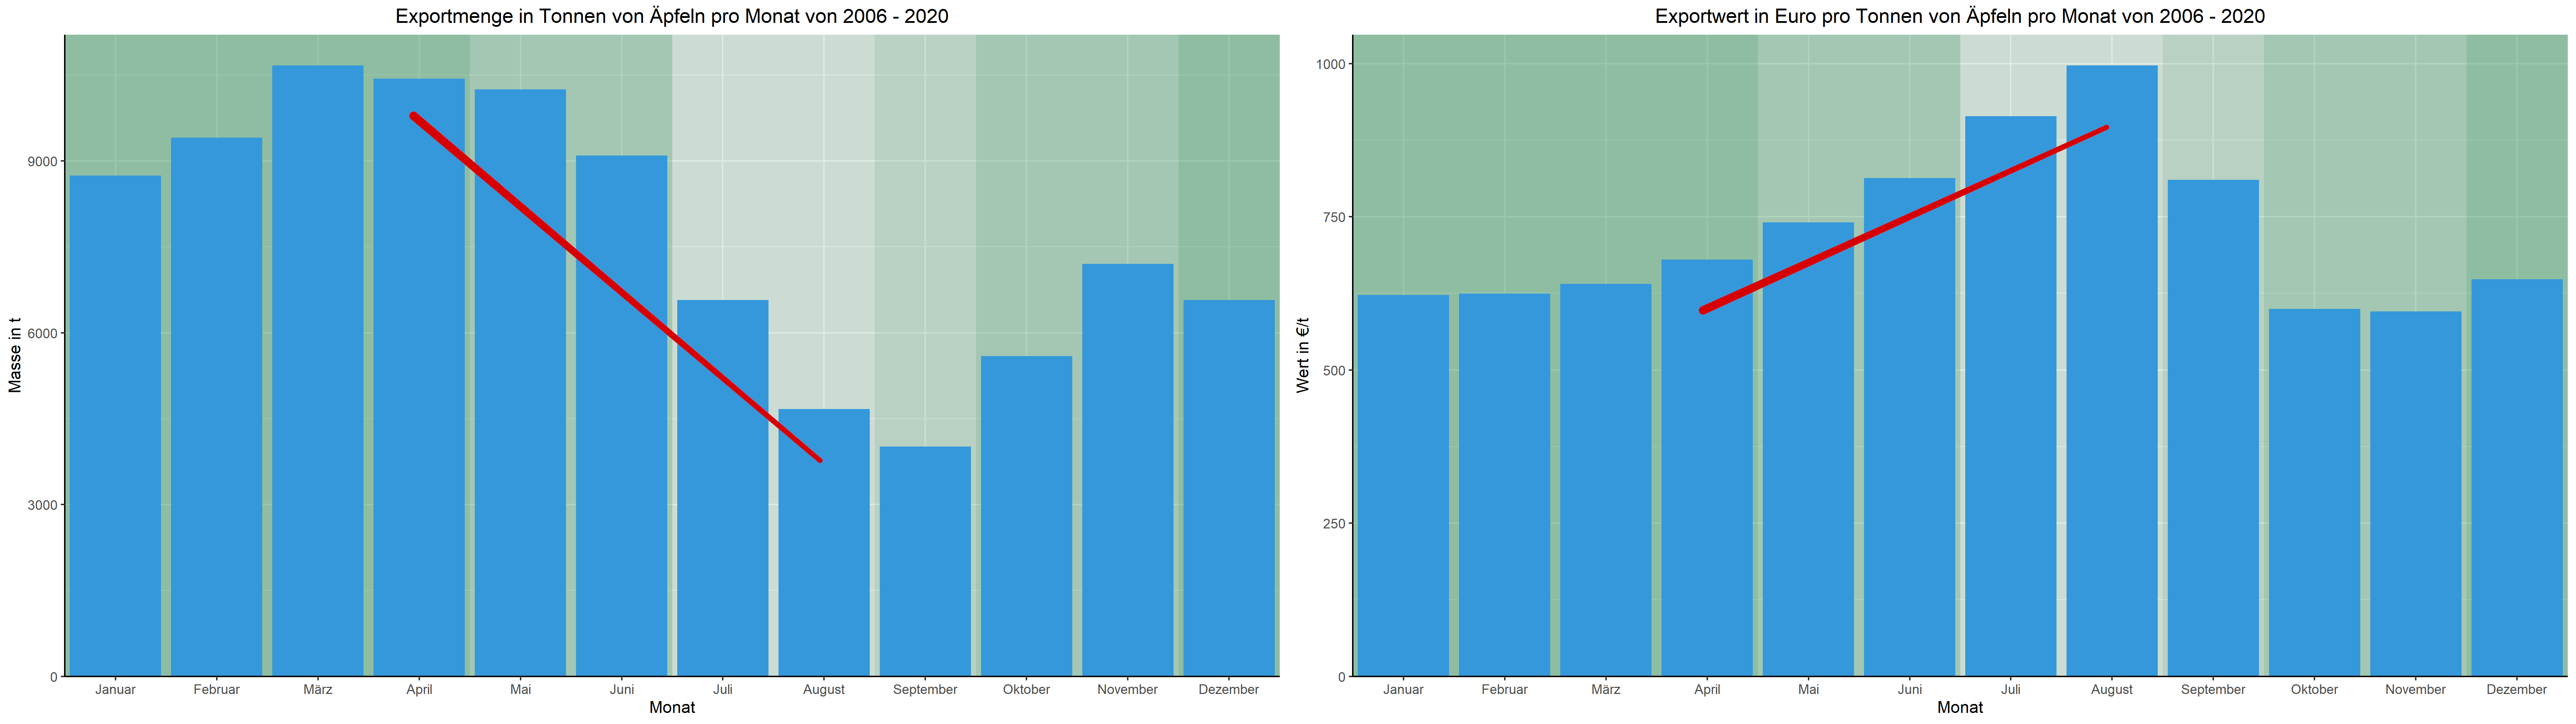
\includegraphics[width=12.5cm]{1_apfel_gegenlaeufig1}
    }
  \end{figure}
\end{frame}

\begin{frame}
\frametitle{Spargel}
  \begin{figure}[h]
    \hbox{\hspace{-1cm}
    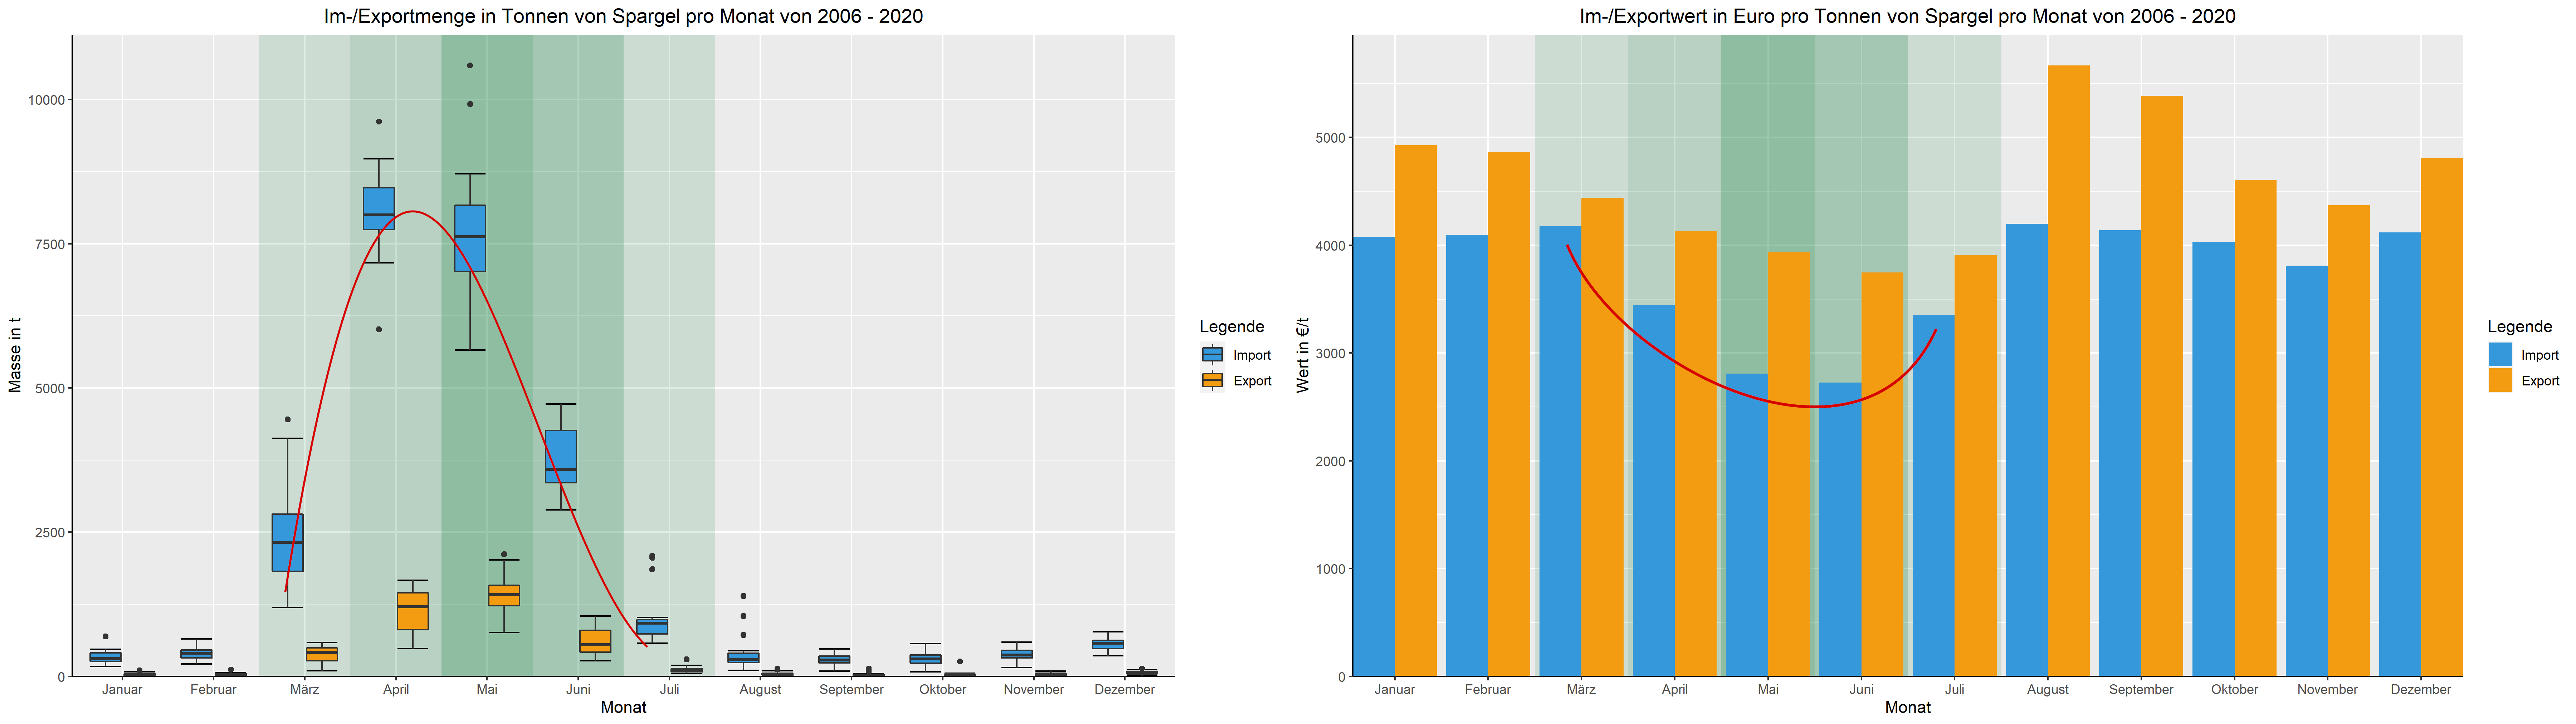
\includegraphics[width=12.5cm]{3_spargel_import2}
    }
  \end{figure}
\end{frame}

\begin{frame}
\frametitle{Orangen}
  \begin{figure}[h]
    \hbox{\hspace{-1cm}
    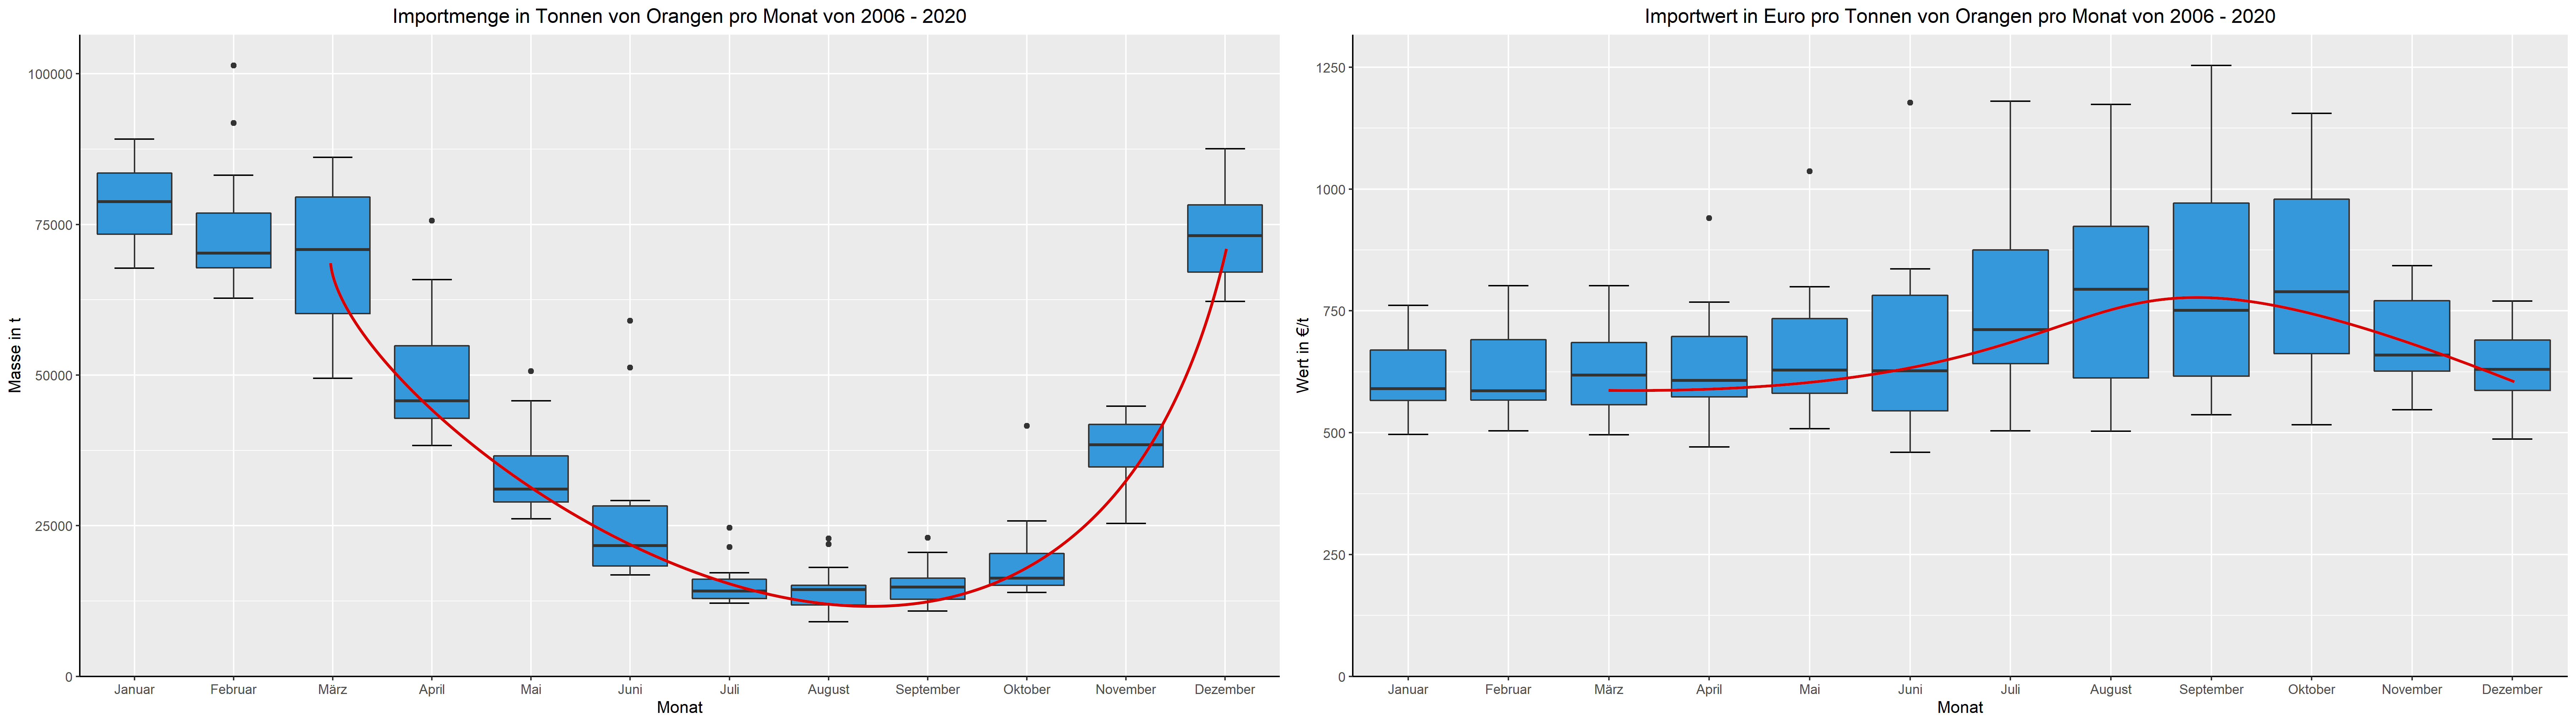
\includegraphics[width=12.5cm]{5_oranges2}
    }
  \end{figure}
\end{frame}

% lisa

\begin{frame}
	\frametitle{Kürbisse}
	\begin{figure}[b]
		\centering
		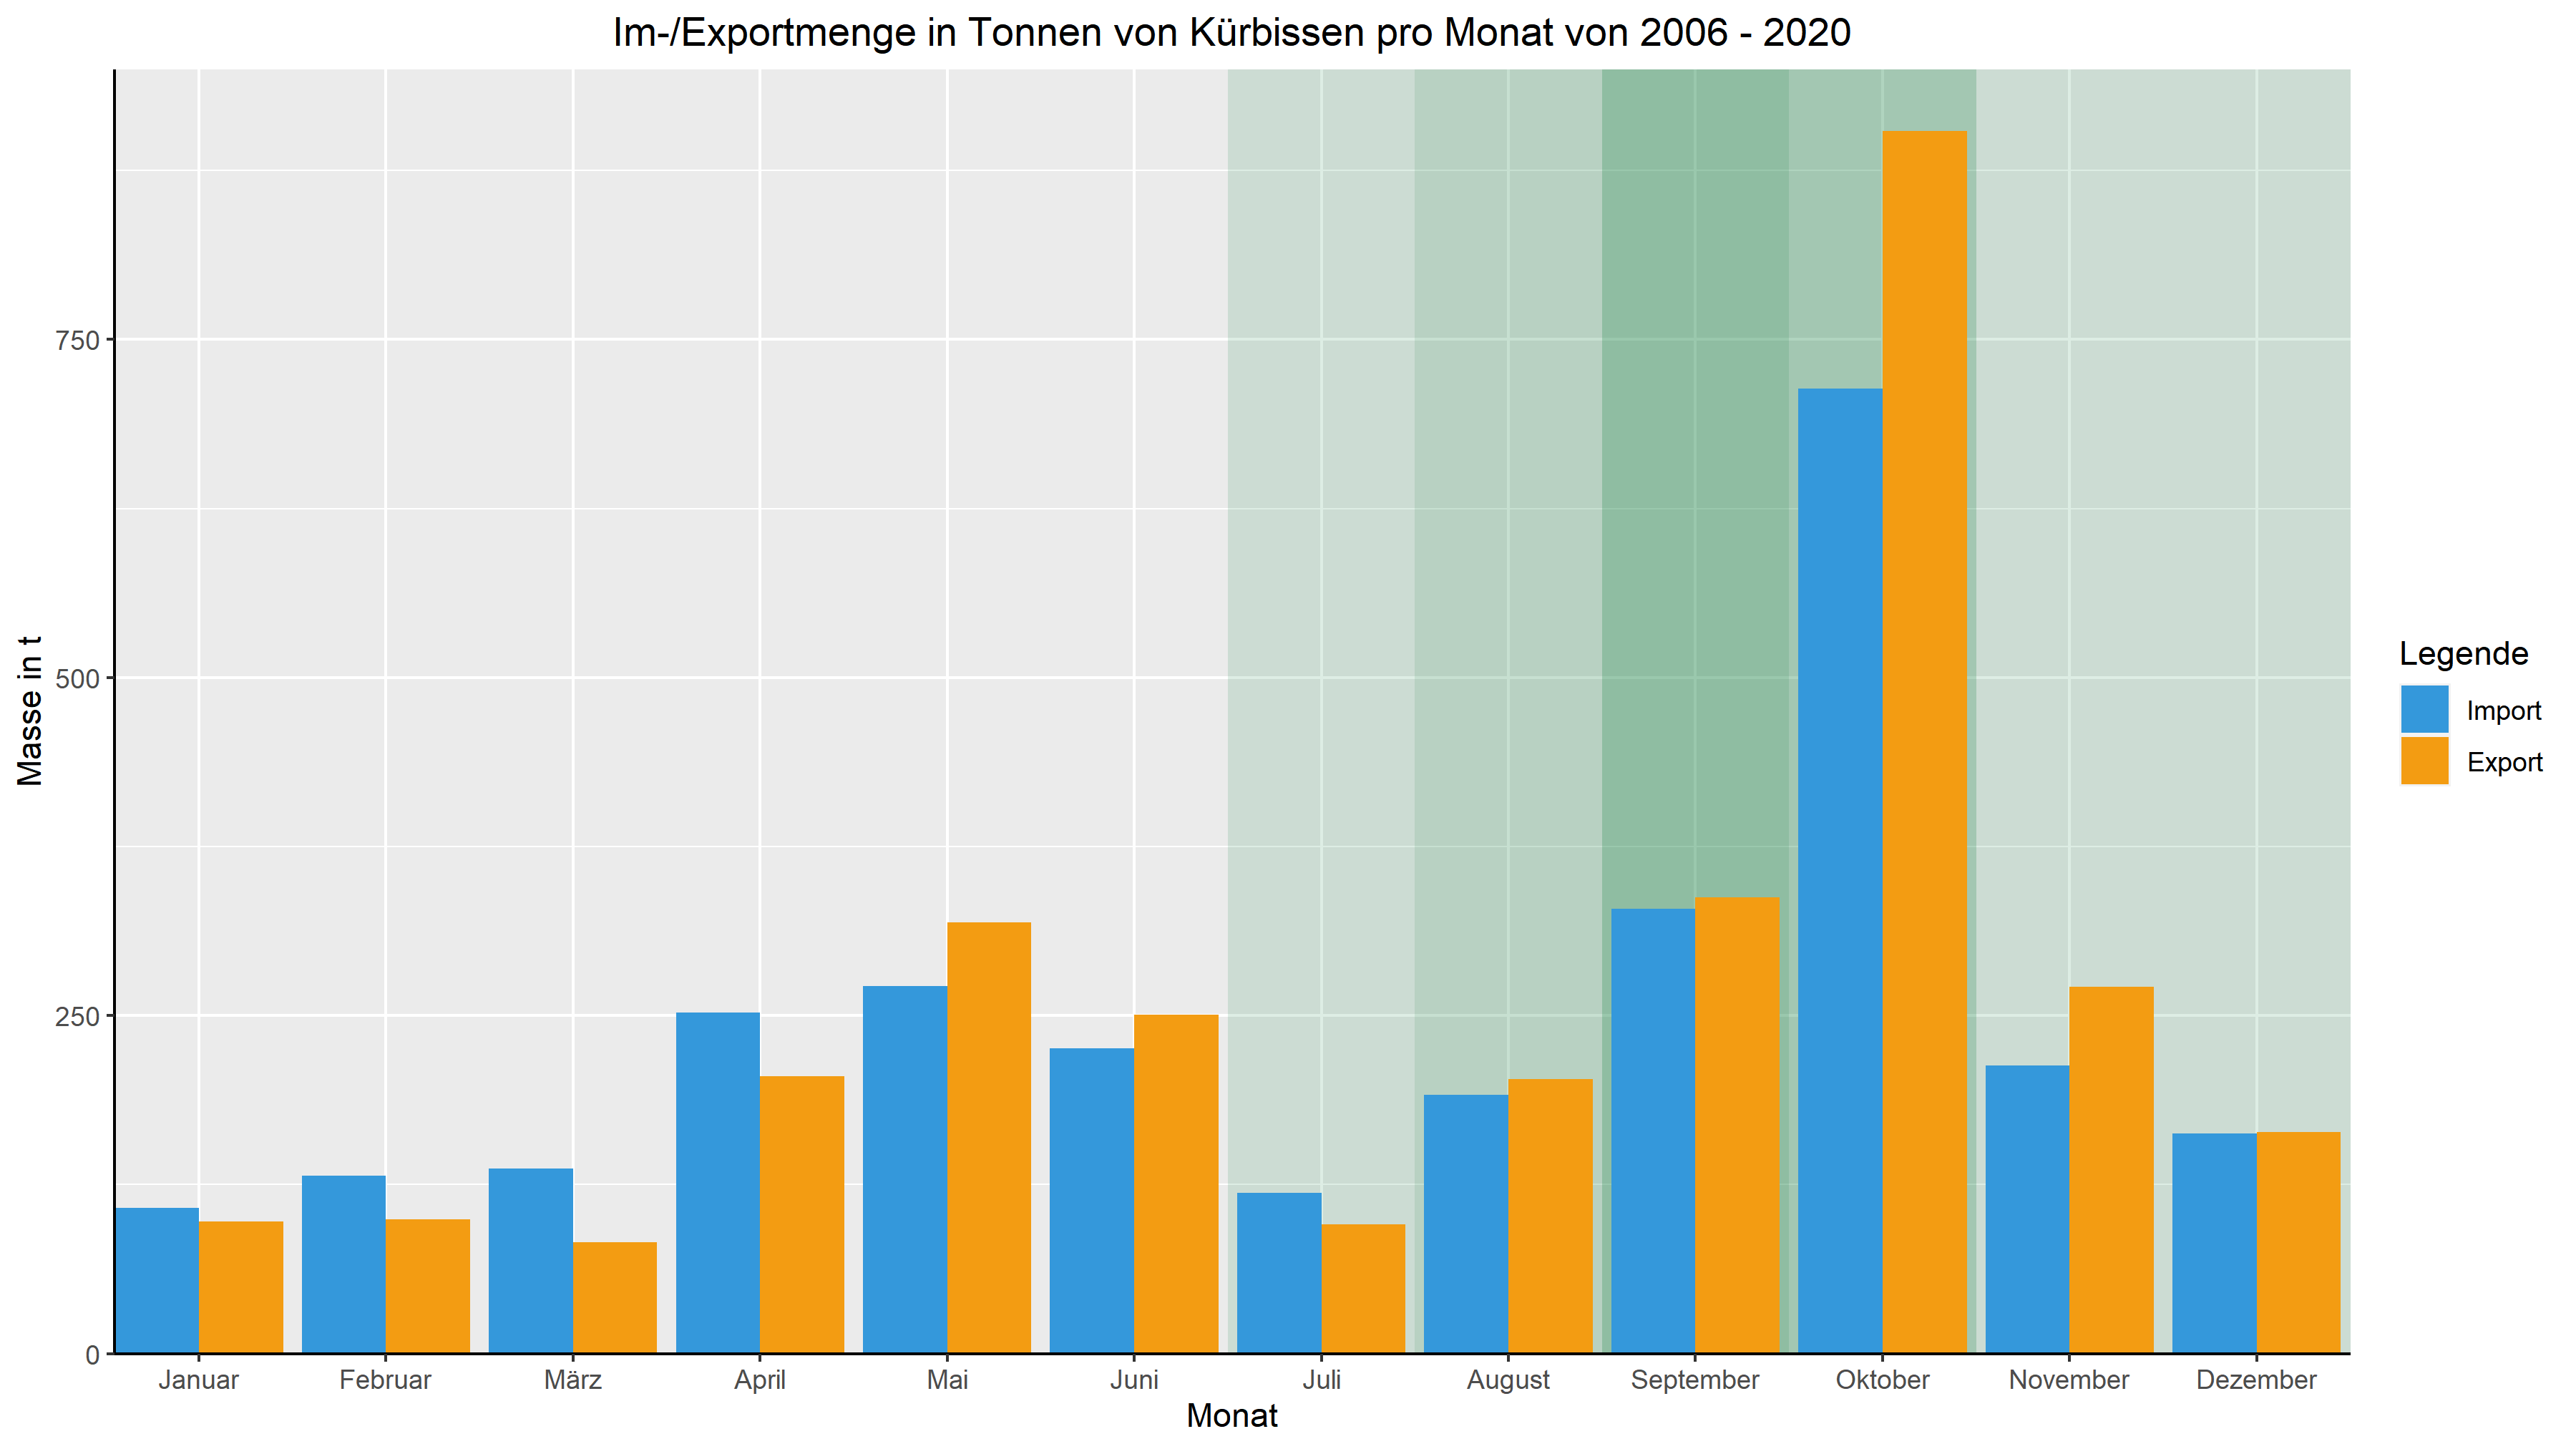
\includegraphics[scale=0.35]{Kuerbissen_monthly_weight_Im-Export}
	\end{figure}
\end{frame}

\begin{frame}
	\frametitle{Kürbisse}
	\begin{figure}[b]
		\centering
		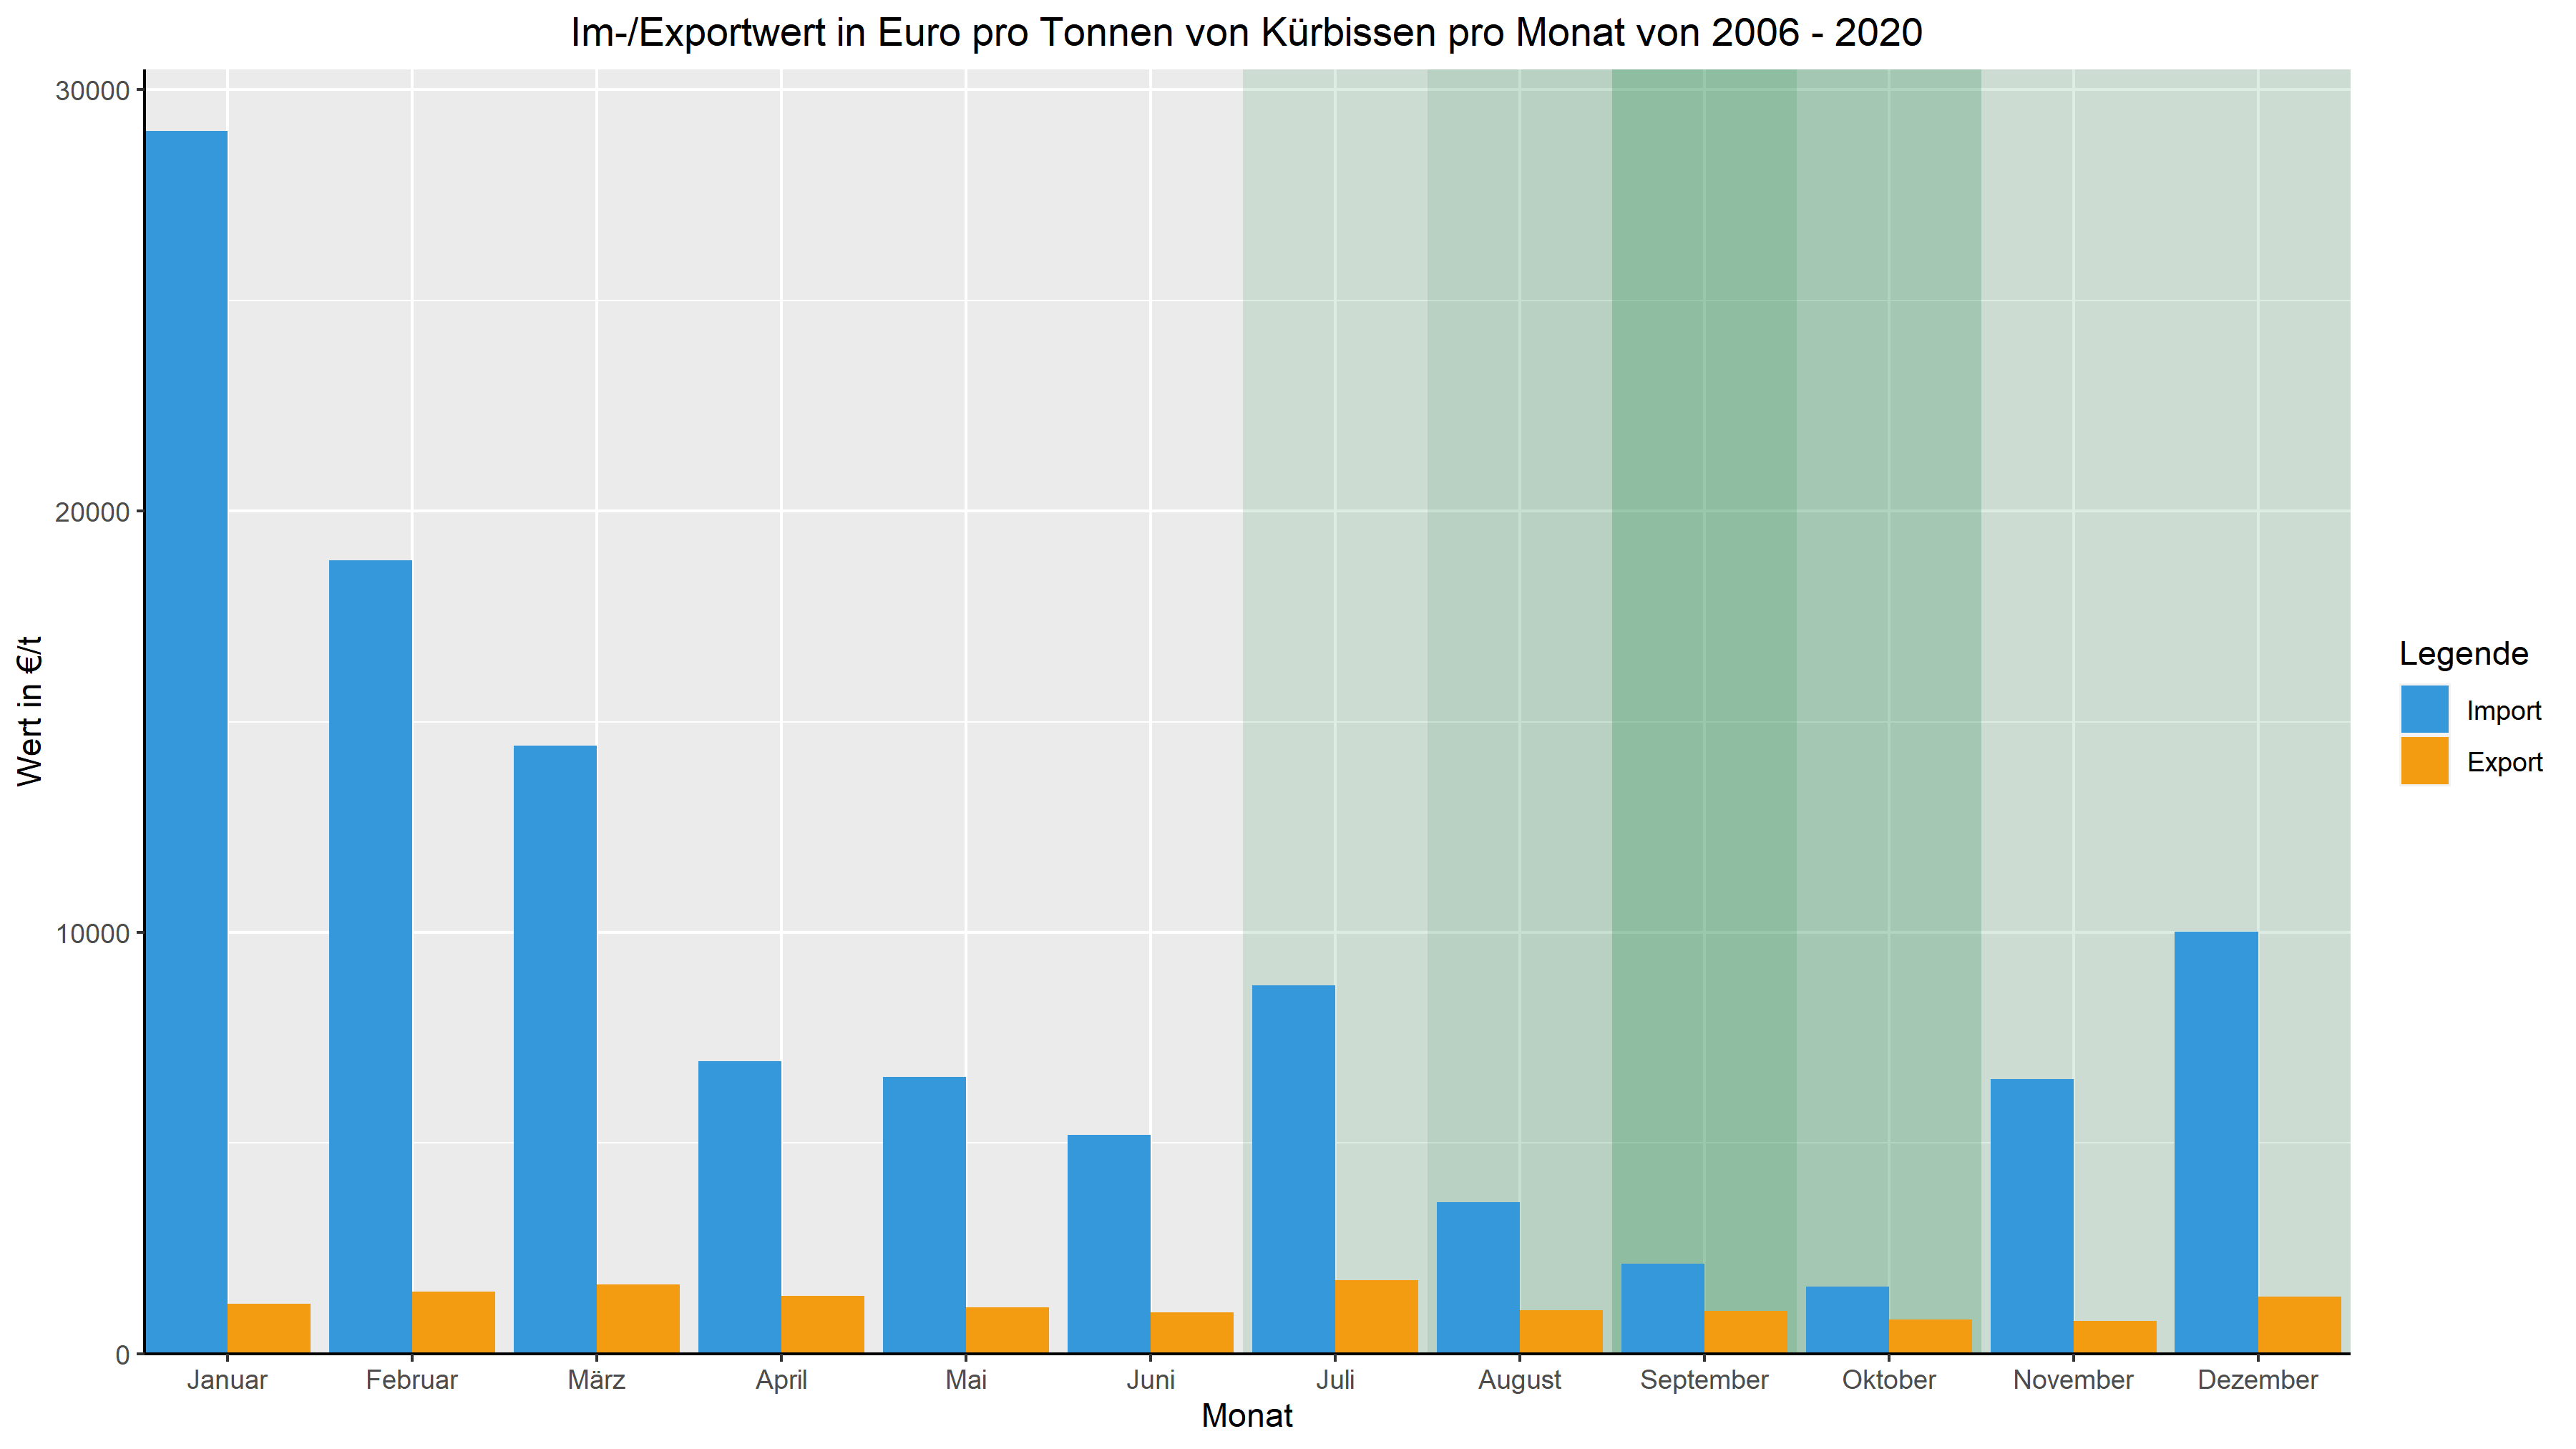
\includegraphics[scale=0.35]{Kuerbissen_monthly_Euro_per_weight_Im-Export}
	\end{figure}
\end{frame}

\section{Fazit}
\begin{frame}
	\frametitle{Fazit}
	\begin{itemize}
		\item Saison eines Produktes beeinflusst Außenhandel
		\item bei Produkten mit längerer Saison/Lagerware weniger Beeinflussung des Außenhandels
		\item Preis sinkt bei starkem Einfluss der Saison
	\end{itemize}
\end{frame}

\begin{frame}
  \frametitle{Fragen?}

  \begin{figure}[h]
    \centering
    \hbox{\hspace{-1cm}
    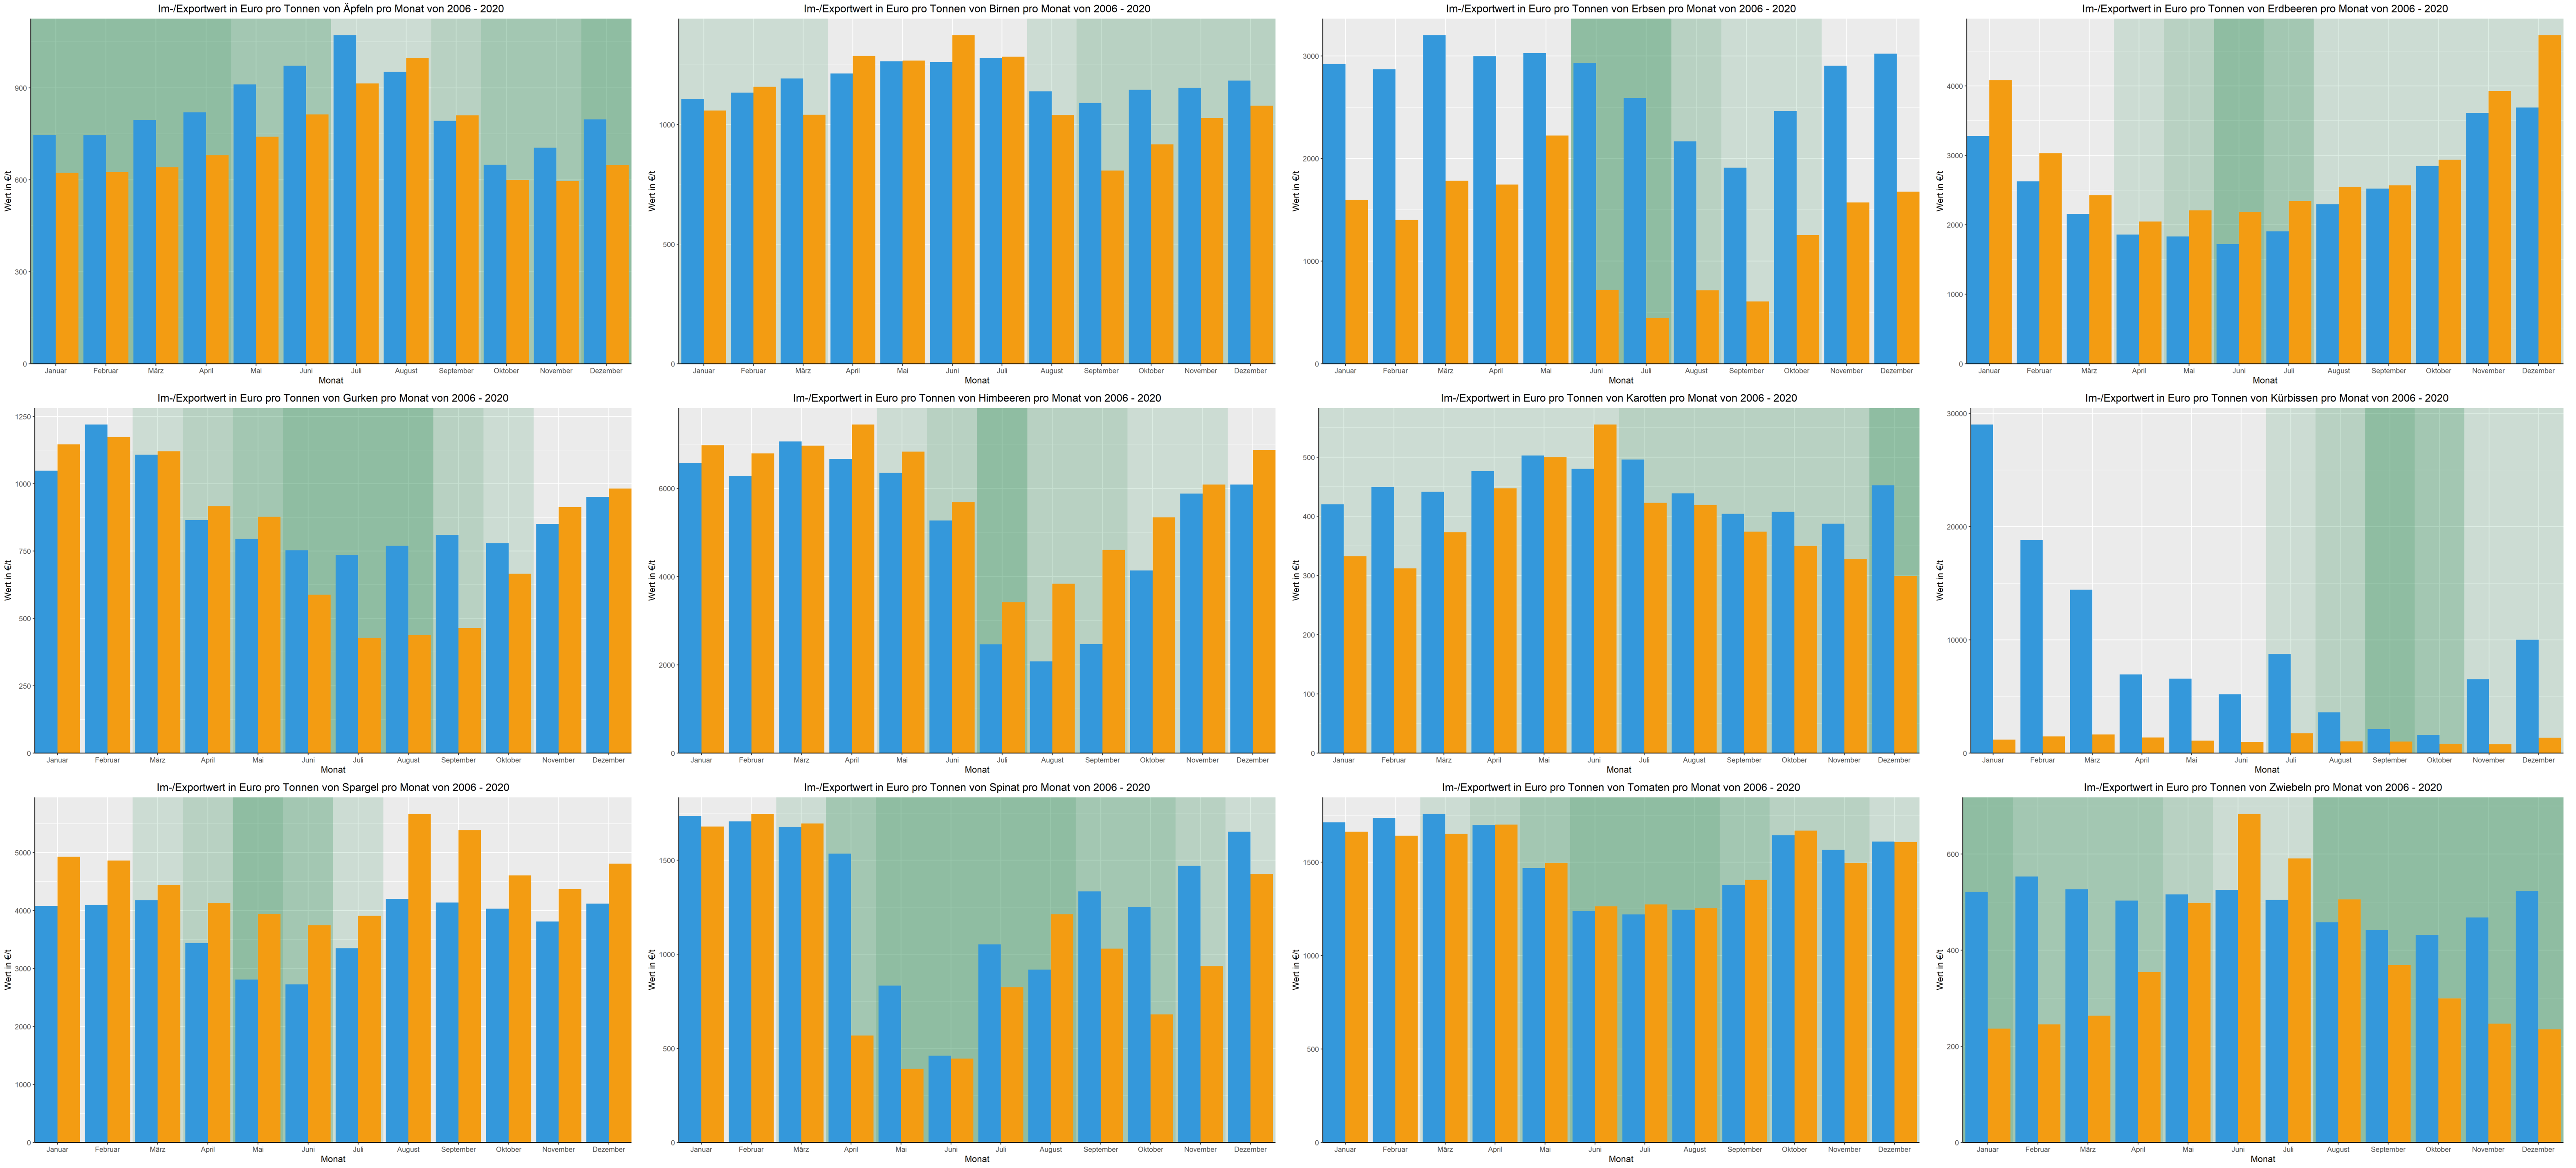
\includegraphics[width=12.5cm]{alle}
    }
    https://github.com/jneidel/htw-gds
  \end{figure}
\end{frame}

\begin{frame}
	\frametitle{Rollenverteilung}
	\begin{description}
		\item[Duc Trung Dao, 575477]Main Data Seeker and Preprocessor
		\item[Jörg Gabele, 571127]Master of Theorie
		\item[Jonathan Neidel, 573619]Projekt Manager
		\item[Marco Neuthor, 573738]Principal Visualizer
		\item[Daniel Spannbauer, 572836]Head of Data Processing
		\item[Lisa-Marlen Wiegandt, 572770]Editor of Chief
	\end{description}
\end{frame}

\begin{frame}
  \frametitle{Quellen}

  \begin{itemize}
    \item Daten: https://www-genesis.destatis.de/genesis/online
    \item Saisonkalender: https://www.bzfe.de/nachhaltiger-konsum/orientierung-beim-einkauf/der-saisonkalender/saisonzeiten-bei-obst-und-gemuese
  \end{itemize}

  % daten quelle
\end{frame}

\end{document}
